\part{Analysis}

A hand digit recognition neural network (HDR-NN) model is implemented in \texttt{C}, \texttt{C++} using Eigen, Python using NumPy, and PyTorch via its \texttt{C++} interface. The performance of HDR-NN training implementations was evaluated on the MCIMX6Q-SDB evaluation board, which was programmed with an Embedded Linux built using the Yocto Project. Model accuracy, execution time, and peak memory usage were compared to gauge the effectiveness of the models. This was examined while altering the number of layers and neurons in each layer. The results of these measurements are presented in the following chapters along with discussions on the obstacles encountered in developing the neural network model and compiling it to operate on the target hardware.

\subsection*{Benchmark Overview}

HDR-NN is implemented in different paradigms, specifically \texttt{C}, \texttt{C++}, Python, and PyTorch. Each of these applications contain a fully connected feedforward neural network composed of multiple layers of neurons connected in a directed graph. The model has a constant input size of 784 which correspond to the 28 x 28 pixel dimensions of the images of the MNIST dataset. The output size of the network is 10, corresponding to the 10 possible digits that the image contains. The number and size of the hidden layers are configurable in each of the different implementations.

The MNIST dataset was selected to train the model, which contains 60,000 training images and 10,000 test images of handwritten digits. The model is trained using stochastic gradient descent, which is an optimization algorithm used to minimize a loss function. The back propagation algorithm is used to calculate the gradients of the loss function with respect to the weights of the network. Finally, the mean square error loss function is used to measure the difference between the predicted output and the actual output of the network. The values of the biases and weights are initialized randomly with the PNGR random generator and a starting seed which are chosen to be identical for the different benchmark applications. The training hyperparameters for the benchmark runs are set to 1 epoch with a batch size of 10, a learning rate of 3, with the network using the sigmoid activation function.

It is essential that the hardware utilized for benchmarking closely resemble the i.MX6 processor on Scania ECUs, as this will make it easier to replicate the experiment on a repurposed ECU and will also provide the most precise results. The MCIMX6Q-SDB evaluation board has four 32-bit Cortex A9 cores. The Cortex A9 core is equipped with ARM V7 instruction set architecture and a powerful VFPv3 floating point unit with NEON SIMD capabilities. The processor has 32 KB instruction and data L1 caches, 1 MB L2 cache and 1 GB DDR3 SDRAM memory. The benchmark applications are designed to be run on a single core of the i.MX6 processor, although it supports quad-core, to ensure the experiment is straightforward and easier to manage. This will also guarantee that the results are precise and accurate.

The Yocto project is used to create an Embedded Linux distribution for the \texttt{imx6qsabresd} machine. The NXP Yocto project guide \cite{nxp-yocto} provides the instructions for building the Linux image, and additional packages such as CMake, python3 are installed during the build. The resulting image file, which used to flash the hardware, has a size of $\sim$ 300Mb.

The accuracy of the model is evaluated after each training epoch on the MNIST test set. After the training of the model for 30 epochs, the final weights and biases of the network and the accuracy on the test set are saved for analysis. This data is used to verify the correctness of the neural network model in each benchmark application.

The GNU time program is a great tool for monitoring the performance of applications. It allows us to measure the execution time and peak memory usage, which is used to compare the effectiveness of training the neural network model on the custom hardware implemented with different paradigms.

A python script was developed to run the experiment, executing each of the benchmark applications (\texttt{C}, \texttt{C++}, Python, PyTorch) one after the other. Every benchmark application is designed to be repeated 10 times, and all the measurements for each of the hidden layer configurations are saved for each of these iterations. The average values of the model accuracy, execution time and peak memory usage across all iterations are utilized for the analysis.

% ============================================
%        Measurement
% ============================================

\chapter{Measurement}

The benchmark applications were executed on an Embedded Linux operating system and the measurements were taken primarily based on the \textit{times} system call and \texttt{perf\_events} Linux API. The primary tools for current measurement values given in the following chapter were taken using the GNU time. GNU Time provides timing statistics such as the elapsed real time between invocation and termination, the user CPU time, and the system CPU time, the later two via the \textit{times} system call API. GNU Time also provides additional information on other resource usage such as the memory, I/O, and IPC calls where available.

The preliminary measurements for the different executions completed with different learning algorithm parameters and model shapes across implementations were timing statistics and maximum resident set size (alternatively referred to as peak memory utilization in the following chapter)

\section{Benchmark Application Parameters}

The benchmark applications all had the same configurable parameters for their learning algorithm and network structure. Initial testing of the different benchmark applications were completed individually with different configurations. These test runs were used to come up with estimates as to how long each run of the training sequence with the different parameters would take and then used to come up with the network shape sizes, and other learning algorithm parameters.

Initially, the network's single hidden layer shape was varied according to powers of two, with the \texttt{C} and \texttt{C++} variants tested with 2, 4, 8, 32, 128, 256, 512, 1024 and so on before adding another hidden layer. The additional hidden layer varied sizes from (16, 16), to (32, 16) and (16, 32), then (128, 16), etc. The final list of shapes and their corresponding shapes for which the measurements results are state in the next chapter are shown in the following table.

\begin{table}[ht]
	\centering
	\begin{tabular}{ |p{11em}|p{14em}| }
		\hline
			\textbf{Hidden layer shape} & \textbf{HDR-NN parameters} (total)\\
		\hline
			2 & 1600 \\
		\hline
			4 & 3190 \\
		\hline
			8 & 6370 \\
		\hline
			16,16 & 13002 \\
		\hline
			32 & 25450 \\
		\hline
			48,48 & 40522 \\
		\hline
			64,16 & 51450 \\
		\hline
			72 & 57250 \\
		\hline
			82,36,16 & 68120 \\
		\hline
			96,96 & 85642 \\
		\hline
			104 & 82690 \\
		\hline
			114 & 90640 \\
		\hline
			128 & 101770 \\
		\hline
	\end{tabular}
\end{table}

The \hyperref[section:hdrnn-ux]{section on UX} in the Design chapter describes how the shape and epochs parameters were configured.

\section{Compilation Options}

All the compiled benchmark programs used the GCC compiler and its \texttt{-O2} optimization flag. Several other optimization opportunities that were possible and tried out however the data present for \texttt{-O2} was fixed for all the applications for uniformity.

The general suite of compiler optimizations from GCC 11.3 are clever enough to use SIMD, inlining, strength reduction, and a suite of powerful optimizations.

\section{Profiling Analysis}

A \texttt{perf\_events} based record was conducted using the \texttt{perf} utility for all the programs. Flame graphs were generated for the same as shown attached in Appendix \hyperref[hdrnn-profile]{III} revealing the areas where the applications were spending the most time on.

\subsection{Memory Profile}

Heaptrack is an alternative to the popular valgrind programming tool for memory profiling that comes under the KDE gear of applications by the KDE community. Heaptrack was used to profile the memory of the benchmark application programs under execution. The resulting graphs are also presented in Appendix \hyperref[hdrnn-memory-profile]{III}


% ============================================
%        Results
% ============================================

\chapter{Results}

This chapter presents the results of the benchmark application runs. The first section contains a brief look at the analysis on the neural network accuracies for the different implementations. The second section considers the performance of the benchmark applications based on execution time and the peak memory usage.

\section{Evaluating Correctness}

As the benchmark applications are developed to be identical by keeping the same structure and configurations, the model accuracy is expected to be similar. Figure \ref{hdrnn-accuracy} showcases that the different implementations perform similarly irrespective of the number of parameters.

\begin{figure}[!ht]
	\centering
	%% Creator: Matplotlib, PGF backend
%%
%% To include the figure in your LaTeX document, write
%%   \input{<filename>.pgf}
%%
%% Make sure the required packages are loaded in your preamble
%%   \usepackage{pgf}
%%
%% Also ensure that all the required font packages are loaded; for instance,
%% the lmodern package is sometimes necessary when using math font.
%%   \usepackage{lmodern}
%%
%% Figures using additional raster images can only be included by \input if
%% they are in the same directory as the main LaTeX file. For loading figures
%% from other directories you can use the `import` package
%%   \usepackage{import}
%%
%% and then include the figures with
%%   \import{<path to file>}{<filename>.pgf}
%%
%% Matplotlib used the following preamble
%%   
%%   \usepackage{fontspec}
%%   \setmainfont{Times New Roman.ttf}[Path=\detokenize{/System/Library/Fonts/Supplemental/}]
%%   \setsansfont{DejaVuSans.ttf}[Path=\detokenize{/opt/homebrew/lib/python3.11/site-packages/matplotlib/mpl-data/fonts/ttf/}]
%%   \setmonofont{DejaVuSansMono.ttf}[Path=\detokenize{/opt/homebrew/lib/python3.11/site-packages/matplotlib/mpl-data/fonts/ttf/}]
%%   \makeatletter\@ifpackageloaded{underscore}{}{\usepackage[strings]{underscore}}\makeatother
%%
\begingroup%
\makeatletter%
\begin{pgfpicture}%
\pgfpathrectangle{\pgfpointorigin}{\pgfqpoint{5.916660in}{5.518849in}}%
\pgfusepath{use as bounding box, clip}%
\begin{pgfscope}%
\pgfsetbuttcap%
\pgfsetmiterjoin%
\definecolor{currentfill}{rgb}{1.000000,1.000000,1.000000}%
\pgfsetfillcolor{currentfill}%
\pgfsetlinewidth{0.000000pt}%
\definecolor{currentstroke}{rgb}{1.000000,1.000000,1.000000}%
\pgfsetstrokecolor{currentstroke}%
\pgfsetdash{}{0pt}%
\pgfpathmoveto{\pgfqpoint{0.000000in}{0.000000in}}%
\pgfpathlineto{\pgfqpoint{5.916660in}{0.000000in}}%
\pgfpathlineto{\pgfqpoint{5.916660in}{5.518849in}}%
\pgfpathlineto{\pgfqpoint{0.000000in}{5.518849in}}%
\pgfpathlineto{\pgfqpoint{0.000000in}{0.000000in}}%
\pgfpathclose%
\pgfusepath{fill}%
\end{pgfscope}%
\begin{pgfscope}%
\pgfsetbuttcap%
\pgfsetmiterjoin%
\definecolor{currentfill}{rgb}{1.000000,1.000000,1.000000}%
\pgfsetfillcolor{currentfill}%
\pgfsetlinewidth{0.000000pt}%
\definecolor{currentstroke}{rgb}{0.000000,0.000000,0.000000}%
\pgfsetstrokecolor{currentstroke}%
\pgfsetstrokeopacity{0.000000}%
\pgfsetdash{}{0pt}%
\pgfpathmoveto{\pgfqpoint{0.587522in}{0.323633in}}%
\pgfpathlineto{\pgfqpoint{5.816660in}{0.323633in}}%
\pgfpathlineto{\pgfqpoint{5.816660in}{4.455361in}}%
\pgfpathlineto{\pgfqpoint{0.587522in}{4.455361in}}%
\pgfpathlineto{\pgfqpoint{0.587522in}{0.323633in}}%
\pgfpathclose%
\pgfusepath{fill}%
\end{pgfscope}%
\begin{pgfscope}%
\pgfpathrectangle{\pgfqpoint{0.587522in}{0.323633in}}{\pgfqpoint{5.229138in}{4.131729in}}%
\pgfusepath{clip}%
\pgfsetbuttcap%
\pgfsetmiterjoin%
\definecolor{currentfill}{rgb}{0.509804,0.792157,0.988235}%
\pgfsetfillcolor{currentfill}%
\pgfsetfillopacity{0.810000}%
\pgfsetlinewidth{0.000000pt}%
\definecolor{currentstroke}{rgb}{0.000000,0.000000,0.000000}%
\pgfsetstrokecolor{currentstroke}%
\pgfsetstrokeopacity{0.810000}%
\pgfsetdash{}{0pt}%
\pgfpathmoveto{\pgfqpoint{0.825210in}{0.323633in}}%
\pgfpathlineto{\pgfqpoint{0.947101in}{0.323633in}}%
\pgfpathlineto{\pgfqpoint{0.947101in}{1.571415in}}%
\pgfpathlineto{\pgfqpoint{0.825210in}{1.571415in}}%
\pgfpathlineto{\pgfqpoint{0.825210in}{0.323633in}}%
\pgfpathclose%
\pgfusepath{fill}%
\end{pgfscope}%
\begin{pgfscope}%
\pgfpathrectangle{\pgfqpoint{0.587522in}{0.323633in}}{\pgfqpoint{5.229138in}{4.131729in}}%
\pgfusepath{clip}%
\pgfsetbuttcap%
\pgfsetmiterjoin%
\definecolor{currentfill}{rgb}{0.509804,0.792157,0.988235}%
\pgfsetfillcolor{currentfill}%
\pgfsetfillopacity{0.810000}%
\pgfsetlinewidth{0.000000pt}%
\definecolor{currentstroke}{rgb}{0.000000,0.000000,0.000000}%
\pgfsetstrokecolor{currentstroke}%
\pgfsetstrokeopacity{0.810000}%
\pgfsetdash{}{0pt}%
\pgfpathmoveto{\pgfqpoint{2.044123in}{0.323633in}}%
\pgfpathlineto{\pgfqpoint{2.166014in}{0.323633in}}%
\pgfpathlineto{\pgfqpoint{2.166014in}{1.513571in}}%
\pgfpathlineto{\pgfqpoint{2.044123in}{1.513571in}}%
\pgfpathlineto{\pgfqpoint{2.044123in}{0.323633in}}%
\pgfpathclose%
\pgfusepath{fill}%
\end{pgfscope}%
\begin{pgfscope}%
\pgfpathrectangle{\pgfqpoint{0.587522in}{0.323633in}}{\pgfqpoint{5.229138in}{4.131729in}}%
\pgfusepath{clip}%
\pgfsetbuttcap%
\pgfsetmiterjoin%
\definecolor{currentfill}{rgb}{0.509804,0.792157,0.988235}%
\pgfsetfillcolor{currentfill}%
\pgfsetfillopacity{0.810000}%
\pgfsetlinewidth{0.000000pt}%
\definecolor{currentstroke}{rgb}{0.000000,0.000000,0.000000}%
\pgfsetstrokecolor{currentstroke}%
\pgfsetstrokeopacity{0.810000}%
\pgfsetdash{}{0pt}%
\pgfpathmoveto{\pgfqpoint{3.263036in}{0.323633in}}%
\pgfpathlineto{\pgfqpoint{3.384928in}{0.323633in}}%
\pgfpathlineto{\pgfqpoint{3.384928in}{2.468000in}}%
\pgfpathlineto{\pgfqpoint{3.263036in}{2.468000in}}%
\pgfpathlineto{\pgfqpoint{3.263036in}{0.323633in}}%
\pgfpathclose%
\pgfusepath{fill}%
\end{pgfscope}%
\begin{pgfscope}%
\pgfpathrectangle{\pgfqpoint{0.587522in}{0.323633in}}{\pgfqpoint{5.229138in}{4.131729in}}%
\pgfusepath{clip}%
\pgfsetbuttcap%
\pgfsetmiterjoin%
\definecolor{currentfill}{rgb}{0.509804,0.792157,0.988235}%
\pgfsetfillcolor{currentfill}%
\pgfsetfillopacity{0.810000}%
\pgfsetlinewidth{0.000000pt}%
\definecolor{currentstroke}{rgb}{0.000000,0.000000,0.000000}%
\pgfsetstrokecolor{currentstroke}%
\pgfsetstrokeopacity{0.810000}%
\pgfsetdash{}{0pt}%
\pgfpathmoveto{\pgfqpoint{4.481950in}{0.323633in}}%
\pgfpathlineto{\pgfqpoint{4.603841in}{0.323633in}}%
\pgfpathlineto{\pgfqpoint{4.603841in}{1.856504in}}%
\pgfpathlineto{\pgfqpoint{4.481950in}{1.856504in}}%
\pgfpathlineto{\pgfqpoint{4.481950in}{0.323633in}}%
\pgfpathclose%
\pgfusepath{fill}%
\end{pgfscope}%
\begin{pgfscope}%
\pgfpathrectangle{\pgfqpoint{0.587522in}{0.323633in}}{\pgfqpoint{5.229138in}{4.131729in}}%
\pgfusepath{clip}%
\pgfsetbuttcap%
\pgfsetmiterjoin%
\definecolor{currentfill}{rgb}{1.000000,0.470588,0.333333}%
\pgfsetfillcolor{currentfill}%
\pgfsetfillopacity{0.810000}%
\pgfsetlinewidth{0.000000pt}%
\definecolor{currentstroke}{rgb}{0.000000,0.000000,0.000000}%
\pgfsetstrokecolor{currentstroke}%
\pgfsetstrokeopacity{0.810000}%
\pgfsetdash{}{0pt}%
\pgfpathmoveto{\pgfqpoint{0.947101in}{0.323633in}}%
\pgfpathlineto{\pgfqpoint{1.068992in}{0.323633in}}%
\pgfpathlineto{\pgfqpoint{1.068992in}{2.637401in}}%
\pgfpathlineto{\pgfqpoint{0.947101in}{2.637401in}}%
\pgfpathlineto{\pgfqpoint{0.947101in}{0.323633in}}%
\pgfpathclose%
\pgfusepath{fill}%
\end{pgfscope}%
\begin{pgfscope}%
\pgfpathrectangle{\pgfqpoint{0.587522in}{0.323633in}}{\pgfqpoint{5.229138in}{4.131729in}}%
\pgfusepath{clip}%
\pgfsetbuttcap%
\pgfsetmiterjoin%
\definecolor{currentfill}{rgb}{1.000000,0.470588,0.333333}%
\pgfsetfillcolor{currentfill}%
\pgfsetfillopacity{0.810000}%
\pgfsetlinewidth{0.000000pt}%
\definecolor{currentstroke}{rgb}{0.000000,0.000000,0.000000}%
\pgfsetstrokecolor{currentstroke}%
\pgfsetstrokeopacity{0.810000}%
\pgfsetdash{}{0pt}%
\pgfpathmoveto{\pgfqpoint{2.166014in}{0.323633in}}%
\pgfpathlineto{\pgfqpoint{2.287906in}{0.323633in}}%
\pgfpathlineto{\pgfqpoint{2.287906in}{3.529854in}}%
\pgfpathlineto{\pgfqpoint{2.166014in}{3.529854in}}%
\pgfpathlineto{\pgfqpoint{2.166014in}{0.323633in}}%
\pgfpathclose%
\pgfusepath{fill}%
\end{pgfscope}%
\begin{pgfscope}%
\pgfpathrectangle{\pgfqpoint{0.587522in}{0.323633in}}{\pgfqpoint{5.229138in}{4.131729in}}%
\pgfusepath{clip}%
\pgfsetbuttcap%
\pgfsetmiterjoin%
\definecolor{currentfill}{rgb}{1.000000,0.470588,0.333333}%
\pgfsetfillcolor{currentfill}%
\pgfsetfillopacity{0.810000}%
\pgfsetlinewidth{0.000000pt}%
\definecolor{currentstroke}{rgb}{0.000000,0.000000,0.000000}%
\pgfsetstrokecolor{currentstroke}%
\pgfsetstrokeopacity{0.810000}%
\pgfsetdash{}{0pt}%
\pgfpathmoveto{\pgfqpoint{3.384928in}{0.323633in}}%
\pgfpathlineto{\pgfqpoint{3.506819in}{0.323633in}}%
\pgfpathlineto{\pgfqpoint{3.506819in}{3.038178in}}%
\pgfpathlineto{\pgfqpoint{3.384928in}{3.038178in}}%
\pgfpathlineto{\pgfqpoint{3.384928in}{0.323633in}}%
\pgfpathclose%
\pgfusepath{fill}%
\end{pgfscope}%
\begin{pgfscope}%
\pgfpathrectangle{\pgfqpoint{0.587522in}{0.323633in}}{\pgfqpoint{5.229138in}{4.131729in}}%
\pgfusepath{clip}%
\pgfsetbuttcap%
\pgfsetmiterjoin%
\definecolor{currentfill}{rgb}{1.000000,0.470588,0.333333}%
\pgfsetfillcolor{currentfill}%
\pgfsetfillopacity{0.810000}%
\pgfsetlinewidth{0.000000pt}%
\definecolor{currentstroke}{rgb}{0.000000,0.000000,0.000000}%
\pgfsetstrokecolor{currentstroke}%
\pgfsetstrokeopacity{0.810000}%
\pgfsetdash{}{0pt}%
\pgfpathmoveto{\pgfqpoint{4.603841in}{0.323633in}}%
\pgfpathlineto{\pgfqpoint{4.725733in}{0.323633in}}%
\pgfpathlineto{\pgfqpoint{4.725733in}{2.703508in}}%
\pgfpathlineto{\pgfqpoint{4.603841in}{2.703508in}}%
\pgfpathlineto{\pgfqpoint{4.603841in}{0.323633in}}%
\pgfpathclose%
\pgfusepath{fill}%
\end{pgfscope}%
\begin{pgfscope}%
\pgfpathrectangle{\pgfqpoint{0.587522in}{0.323633in}}{\pgfqpoint{5.229138in}{4.131729in}}%
\pgfusepath{clip}%
\pgfsetbuttcap%
\pgfsetmiterjoin%
\definecolor{currentfill}{rgb}{0.121569,0.654902,0.454902}%
\pgfsetfillcolor{currentfill}%
\pgfsetfillopacity{0.810000}%
\pgfsetlinewidth{0.000000pt}%
\definecolor{currentstroke}{rgb}{0.000000,0.000000,0.000000}%
\pgfsetstrokecolor{currentstroke}%
\pgfsetstrokeopacity{0.810000}%
\pgfsetdash{}{0pt}%
\pgfpathmoveto{\pgfqpoint{1.068992in}{0.323633in}}%
\pgfpathlineto{\pgfqpoint{1.190884in}{0.323633in}}%
\pgfpathlineto{\pgfqpoint{1.190884in}{3.971949in}}%
\pgfpathlineto{\pgfqpoint{1.068992in}{3.971949in}}%
\pgfpathlineto{\pgfqpoint{1.068992in}{0.323633in}}%
\pgfpathclose%
\pgfusepath{fill}%
\end{pgfscope}%
\begin{pgfscope}%
\pgfpathrectangle{\pgfqpoint{0.587522in}{0.323633in}}{\pgfqpoint{5.229138in}{4.131729in}}%
\pgfusepath{clip}%
\pgfsetbuttcap%
\pgfsetmiterjoin%
\definecolor{currentfill}{rgb}{0.121569,0.654902,0.454902}%
\pgfsetfillcolor{currentfill}%
\pgfsetfillopacity{0.810000}%
\pgfsetlinewidth{0.000000pt}%
\definecolor{currentstroke}{rgb}{0.000000,0.000000,0.000000}%
\pgfsetstrokecolor{currentstroke}%
\pgfsetstrokeopacity{0.810000}%
\pgfsetdash{}{0pt}%
\pgfpathmoveto{\pgfqpoint{2.287906in}{0.323633in}}%
\pgfpathlineto{\pgfqpoint{2.409797in}{0.323633in}}%
\pgfpathlineto{\pgfqpoint{2.409797in}{3.922368in}}%
\pgfpathlineto{\pgfqpoint{2.287906in}{3.922368in}}%
\pgfpathlineto{\pgfqpoint{2.287906in}{0.323633in}}%
\pgfpathclose%
\pgfusepath{fill}%
\end{pgfscope}%
\begin{pgfscope}%
\pgfpathrectangle{\pgfqpoint{0.587522in}{0.323633in}}{\pgfqpoint{5.229138in}{4.131729in}}%
\pgfusepath{clip}%
\pgfsetbuttcap%
\pgfsetmiterjoin%
\definecolor{currentfill}{rgb}{0.121569,0.654902,0.454902}%
\pgfsetfillcolor{currentfill}%
\pgfsetfillopacity{0.810000}%
\pgfsetlinewidth{0.000000pt}%
\definecolor{currentstroke}{rgb}{0.000000,0.000000,0.000000}%
\pgfsetstrokecolor{currentstroke}%
\pgfsetstrokeopacity{0.810000}%
\pgfsetdash{}{0pt}%
\pgfpathmoveto{\pgfqpoint{3.506819in}{0.323633in}}%
\pgfpathlineto{\pgfqpoint{3.628710in}{0.323633in}}%
\pgfpathlineto{\pgfqpoint{3.628710in}{4.079374in}}%
\pgfpathlineto{\pgfqpoint{3.506819in}{4.079374in}}%
\pgfpathlineto{\pgfqpoint{3.506819in}{0.323633in}}%
\pgfpathclose%
\pgfusepath{fill}%
\end{pgfscope}%
\begin{pgfscope}%
\pgfpathrectangle{\pgfqpoint{0.587522in}{0.323633in}}{\pgfqpoint{5.229138in}{4.131729in}}%
\pgfusepath{clip}%
\pgfsetbuttcap%
\pgfsetmiterjoin%
\definecolor{currentfill}{rgb}{0.121569,0.654902,0.454902}%
\pgfsetfillcolor{currentfill}%
\pgfsetfillopacity{0.810000}%
\pgfsetlinewidth{0.000000pt}%
\definecolor{currentstroke}{rgb}{0.000000,0.000000,0.000000}%
\pgfsetstrokecolor{currentstroke}%
\pgfsetstrokeopacity{0.810000}%
\pgfsetdash{}{0pt}%
\pgfpathmoveto{\pgfqpoint{4.725733in}{0.323633in}}%
\pgfpathlineto{\pgfqpoint{4.847624in}{0.323633in}}%
\pgfpathlineto{\pgfqpoint{4.847624in}{3.996740in}}%
\pgfpathlineto{\pgfqpoint{4.725733in}{3.996740in}}%
\pgfpathlineto{\pgfqpoint{4.725733in}{0.323633in}}%
\pgfpathclose%
\pgfusepath{fill}%
\end{pgfscope}%
\begin{pgfscope}%
\pgfpathrectangle{\pgfqpoint{0.587522in}{0.323633in}}{\pgfqpoint{5.229138in}{4.131729in}}%
\pgfusepath{clip}%
\pgfsetbuttcap%
\pgfsetmiterjoin%
\definecolor{currentfill}{rgb}{0.984314,0.160784,0.262745}%
\pgfsetfillcolor{currentfill}%
\pgfsetfillopacity{0.810000}%
\pgfsetlinewidth{0.000000pt}%
\definecolor{currentstroke}{rgb}{0.000000,0.000000,0.000000}%
\pgfsetstrokecolor{currentstroke}%
\pgfsetstrokeopacity{0.810000}%
\pgfsetdash{}{0pt}%
\pgfpathmoveto{\pgfqpoint{1.190884in}{0.323633in}}%
\pgfpathlineto{\pgfqpoint{1.312775in}{0.323633in}}%
\pgfpathlineto{\pgfqpoint{1.312775in}{4.120691in}}%
\pgfpathlineto{\pgfqpoint{1.190884in}{4.120691in}}%
\pgfpathlineto{\pgfqpoint{1.190884in}{0.323633in}}%
\pgfpathclose%
\pgfusepath{fill}%
\end{pgfscope}%
\begin{pgfscope}%
\pgfpathrectangle{\pgfqpoint{0.587522in}{0.323633in}}{\pgfqpoint{5.229138in}{4.131729in}}%
\pgfusepath{clip}%
\pgfsetbuttcap%
\pgfsetmiterjoin%
\definecolor{currentfill}{rgb}{0.984314,0.160784,0.262745}%
\pgfsetfillcolor{currentfill}%
\pgfsetfillopacity{0.810000}%
\pgfsetlinewidth{0.000000pt}%
\definecolor{currentstroke}{rgb}{0.000000,0.000000,0.000000}%
\pgfsetstrokecolor{currentstroke}%
\pgfsetstrokeopacity{0.810000}%
\pgfsetdash{}{0pt}%
\pgfpathmoveto{\pgfqpoint{2.409797in}{0.323633in}}%
\pgfpathlineto{\pgfqpoint{2.531688in}{0.323633in}}%
\pgfpathlineto{\pgfqpoint{2.531688in}{4.112428in}}%
\pgfpathlineto{\pgfqpoint{2.409797in}{4.112428in}}%
\pgfpathlineto{\pgfqpoint{2.409797in}{0.323633in}}%
\pgfpathclose%
\pgfusepath{fill}%
\end{pgfscope}%
\begin{pgfscope}%
\pgfpathrectangle{\pgfqpoint{0.587522in}{0.323633in}}{\pgfqpoint{5.229138in}{4.131729in}}%
\pgfusepath{clip}%
\pgfsetbuttcap%
\pgfsetmiterjoin%
\definecolor{currentfill}{rgb}{0.984314,0.160784,0.262745}%
\pgfsetfillcolor{currentfill}%
\pgfsetfillopacity{0.810000}%
\pgfsetlinewidth{0.000000pt}%
\definecolor{currentstroke}{rgb}{0.000000,0.000000,0.000000}%
\pgfsetstrokecolor{currentstroke}%
\pgfsetstrokeopacity{0.810000}%
\pgfsetdash{}{0pt}%
\pgfpathmoveto{\pgfqpoint{3.628710in}{0.323633in}}%
\pgfpathlineto{\pgfqpoint{3.750602in}{0.323633in}}%
\pgfpathlineto{\pgfqpoint{3.750602in}{4.190931in}}%
\pgfpathlineto{\pgfqpoint{3.628710in}{4.190931in}}%
\pgfpathlineto{\pgfqpoint{3.628710in}{0.323633in}}%
\pgfpathclose%
\pgfusepath{fill}%
\end{pgfscope}%
\begin{pgfscope}%
\pgfpathrectangle{\pgfqpoint{0.587522in}{0.323633in}}{\pgfqpoint{5.229138in}{4.131729in}}%
\pgfusepath{clip}%
\pgfsetbuttcap%
\pgfsetmiterjoin%
\definecolor{currentfill}{rgb}{0.984314,0.160784,0.262745}%
\pgfsetfillcolor{currentfill}%
\pgfsetfillopacity{0.810000}%
\pgfsetlinewidth{0.000000pt}%
\definecolor{currentstroke}{rgb}{0.000000,0.000000,0.000000}%
\pgfsetstrokecolor{currentstroke}%
\pgfsetstrokeopacity{0.810000}%
\pgfsetdash{}{0pt}%
\pgfpathmoveto{\pgfqpoint{4.847624in}{0.323633in}}%
\pgfpathlineto{\pgfqpoint{4.969515in}{0.323633in}}%
\pgfpathlineto{\pgfqpoint{4.969515in}{4.124823in}}%
\pgfpathlineto{\pgfqpoint{4.847624in}{4.124823in}}%
\pgfpathlineto{\pgfqpoint{4.847624in}{0.323633in}}%
\pgfpathclose%
\pgfusepath{fill}%
\end{pgfscope}%
\begin{pgfscope}%
\pgfpathrectangle{\pgfqpoint{0.587522in}{0.323633in}}{\pgfqpoint{5.229138in}{4.131729in}}%
\pgfusepath{clip}%
\pgfsetbuttcap%
\pgfsetmiterjoin%
\definecolor{currentfill}{rgb}{0.607843,0.372549,0.752941}%
\pgfsetfillcolor{currentfill}%
\pgfsetfillopacity{0.810000}%
\pgfsetlinewidth{0.000000pt}%
\definecolor{currentstroke}{rgb}{0.000000,0.000000,0.000000}%
\pgfsetstrokecolor{currentstroke}%
\pgfsetstrokeopacity{0.810000}%
\pgfsetdash{}{0pt}%
\pgfpathmoveto{\pgfqpoint{1.312775in}{0.323633in}}%
\pgfpathlineto{\pgfqpoint{1.434666in}{0.323633in}}%
\pgfpathlineto{\pgfqpoint{1.434666in}{4.211589in}}%
\pgfpathlineto{\pgfqpoint{1.312775in}{4.211589in}}%
\pgfpathlineto{\pgfqpoint{1.312775in}{0.323633in}}%
\pgfpathclose%
\pgfusepath{fill}%
\end{pgfscope}%
\begin{pgfscope}%
\pgfpathrectangle{\pgfqpoint{0.587522in}{0.323633in}}{\pgfqpoint{5.229138in}{4.131729in}}%
\pgfusepath{clip}%
\pgfsetbuttcap%
\pgfsetmiterjoin%
\definecolor{currentfill}{rgb}{0.607843,0.372549,0.752941}%
\pgfsetfillcolor{currentfill}%
\pgfsetfillopacity{0.810000}%
\pgfsetlinewidth{0.000000pt}%
\definecolor{currentstroke}{rgb}{0.000000,0.000000,0.000000}%
\pgfsetstrokecolor{currentstroke}%
\pgfsetstrokeopacity{0.810000}%
\pgfsetdash{}{0pt}%
\pgfpathmoveto{\pgfqpoint{2.531688in}{0.323633in}}%
\pgfpathlineto{\pgfqpoint{2.653580in}{0.323633in}}%
\pgfpathlineto{\pgfqpoint{2.653580in}{4.203326in}}%
\pgfpathlineto{\pgfqpoint{2.531688in}{4.203326in}}%
\pgfpathlineto{\pgfqpoint{2.531688in}{0.323633in}}%
\pgfpathclose%
\pgfusepath{fill}%
\end{pgfscope}%
\begin{pgfscope}%
\pgfpathrectangle{\pgfqpoint{0.587522in}{0.323633in}}{\pgfqpoint{5.229138in}{4.131729in}}%
\pgfusepath{clip}%
\pgfsetbuttcap%
\pgfsetmiterjoin%
\definecolor{currentfill}{rgb}{0.607843,0.372549,0.752941}%
\pgfsetfillcolor{currentfill}%
\pgfsetfillopacity{0.810000}%
\pgfsetlinewidth{0.000000pt}%
\definecolor{currentstroke}{rgb}{0.000000,0.000000,0.000000}%
\pgfsetstrokecolor{currentstroke}%
\pgfsetstrokeopacity{0.810000}%
\pgfsetdash{}{0pt}%
\pgfpathmoveto{\pgfqpoint{3.750602in}{0.323633in}}%
\pgfpathlineto{\pgfqpoint{3.872493in}{0.323633in}}%
\pgfpathlineto{\pgfqpoint{3.872493in}{4.265302in}}%
\pgfpathlineto{\pgfqpoint{3.750602in}{4.265302in}}%
\pgfpathlineto{\pgfqpoint{3.750602in}{0.323633in}}%
\pgfpathclose%
\pgfusepath{fill}%
\end{pgfscope}%
\begin{pgfscope}%
\pgfpathrectangle{\pgfqpoint{0.587522in}{0.323633in}}{\pgfqpoint{5.229138in}{4.131729in}}%
\pgfusepath{clip}%
\pgfsetbuttcap%
\pgfsetmiterjoin%
\definecolor{currentfill}{rgb}{0.607843,0.372549,0.752941}%
\pgfsetfillcolor{currentfill}%
\pgfsetfillopacity{0.810000}%
\pgfsetlinewidth{0.000000pt}%
\definecolor{currentstroke}{rgb}{0.000000,0.000000,0.000000}%
\pgfsetstrokecolor{currentstroke}%
\pgfsetstrokeopacity{0.810000}%
\pgfsetdash{}{0pt}%
\pgfpathmoveto{\pgfqpoint{4.969515in}{0.323633in}}%
\pgfpathlineto{\pgfqpoint{5.091407in}{0.323633in}}%
\pgfpathlineto{\pgfqpoint{5.091407in}{3.847997in}}%
\pgfpathlineto{\pgfqpoint{4.969515in}{3.847997in}}%
\pgfpathlineto{\pgfqpoint{4.969515in}{0.323633in}}%
\pgfpathclose%
\pgfusepath{fill}%
\end{pgfscope}%
\begin{pgfscope}%
\pgfpathrectangle{\pgfqpoint{0.587522in}{0.323633in}}{\pgfqpoint{5.229138in}{4.131729in}}%
\pgfusepath{clip}%
\pgfsetbuttcap%
\pgfsetmiterjoin%
\definecolor{currentfill}{rgb}{0.529412,0.372549,0.258824}%
\pgfsetfillcolor{currentfill}%
\pgfsetfillopacity{0.810000}%
\pgfsetlinewidth{0.000000pt}%
\definecolor{currentstroke}{rgb}{0.000000,0.000000,0.000000}%
\pgfsetstrokecolor{currentstroke}%
\pgfsetstrokeopacity{0.810000}%
\pgfsetdash{}{0pt}%
\pgfpathmoveto{\pgfqpoint{1.434666in}{0.323633in}}%
\pgfpathlineto{\pgfqpoint{1.556558in}{0.323633in}}%
\pgfpathlineto{\pgfqpoint{1.556558in}{4.100033in}}%
\pgfpathlineto{\pgfqpoint{1.434666in}{4.100033in}}%
\pgfpathlineto{\pgfqpoint{1.434666in}{0.323633in}}%
\pgfpathclose%
\pgfusepath{fill}%
\end{pgfscope}%
\begin{pgfscope}%
\pgfpathrectangle{\pgfqpoint{0.587522in}{0.323633in}}{\pgfqpoint{5.229138in}{4.131729in}}%
\pgfusepath{clip}%
\pgfsetbuttcap%
\pgfsetmiterjoin%
\definecolor{currentfill}{rgb}{0.529412,0.372549,0.258824}%
\pgfsetfillcolor{currentfill}%
\pgfsetfillopacity{0.810000}%
\pgfsetlinewidth{0.000000pt}%
\definecolor{currentstroke}{rgb}{0.000000,0.000000,0.000000}%
\pgfsetstrokecolor{currentstroke}%
\pgfsetstrokeopacity{0.810000}%
\pgfsetdash{}{0pt}%
\pgfpathmoveto{\pgfqpoint{2.653580in}{0.323633in}}%
\pgfpathlineto{\pgfqpoint{2.775471in}{0.323633in}}%
\pgfpathlineto{\pgfqpoint{2.775471in}{4.182667in}}%
\pgfpathlineto{\pgfqpoint{2.653580in}{4.182667in}}%
\pgfpathlineto{\pgfqpoint{2.653580in}{0.323633in}}%
\pgfpathclose%
\pgfusepath{fill}%
\end{pgfscope}%
\begin{pgfscope}%
\pgfpathrectangle{\pgfqpoint{0.587522in}{0.323633in}}{\pgfqpoint{5.229138in}{4.131729in}}%
\pgfusepath{clip}%
\pgfsetbuttcap%
\pgfsetmiterjoin%
\definecolor{currentfill}{rgb}{0.529412,0.372549,0.258824}%
\pgfsetfillcolor{currentfill}%
\pgfsetfillopacity{0.810000}%
\pgfsetlinewidth{0.000000pt}%
\definecolor{currentstroke}{rgb}{0.000000,0.000000,0.000000}%
\pgfsetstrokecolor{currentstroke}%
\pgfsetstrokeopacity{0.810000}%
\pgfsetdash{}{0pt}%
\pgfpathmoveto{\pgfqpoint{3.872493in}{0.323633in}}%
\pgfpathlineto{\pgfqpoint{3.994384in}{0.323633in}}%
\pgfpathlineto{\pgfqpoint{3.994384in}{4.025662in}}%
\pgfpathlineto{\pgfqpoint{3.872493in}{4.025662in}}%
\pgfpathlineto{\pgfqpoint{3.872493in}{0.323633in}}%
\pgfpathclose%
\pgfusepath{fill}%
\end{pgfscope}%
\begin{pgfscope}%
\pgfpathrectangle{\pgfqpoint{0.587522in}{0.323633in}}{\pgfqpoint{5.229138in}{4.131729in}}%
\pgfusepath{clip}%
\pgfsetbuttcap%
\pgfsetmiterjoin%
\definecolor{currentfill}{rgb}{0.529412,0.372549,0.258824}%
\pgfsetfillcolor{currentfill}%
\pgfsetfillopacity{0.810000}%
\pgfsetlinewidth{0.000000pt}%
\definecolor{currentstroke}{rgb}{0.000000,0.000000,0.000000}%
\pgfsetstrokecolor{currentstroke}%
\pgfsetstrokeopacity{0.810000}%
\pgfsetdash{}{0pt}%
\pgfpathmoveto{\pgfqpoint{5.091407in}{0.323633in}}%
\pgfpathlineto{\pgfqpoint{5.213298in}{0.323633in}}%
\pgfpathlineto{\pgfqpoint{5.213298in}{4.178536in}}%
\pgfpathlineto{\pgfqpoint{5.091407in}{4.178536in}}%
\pgfpathlineto{\pgfqpoint{5.091407in}{0.323633in}}%
\pgfpathclose%
\pgfusepath{fill}%
\end{pgfscope}%
\begin{pgfscope}%
\pgfpathrectangle{\pgfqpoint{0.587522in}{0.323633in}}{\pgfqpoint{5.229138in}{4.131729in}}%
\pgfusepath{clip}%
\pgfsetbuttcap%
\pgfsetmiterjoin%
\definecolor{currentfill}{rgb}{0.964706,0.407843,0.556863}%
\pgfsetfillcolor{currentfill}%
\pgfsetfillopacity{0.810000}%
\pgfsetlinewidth{0.000000pt}%
\definecolor{currentstroke}{rgb}{0.000000,0.000000,0.000000}%
\pgfsetstrokecolor{currentstroke}%
\pgfsetstrokeopacity{0.810000}%
\pgfsetdash{}{0pt}%
\pgfpathmoveto{\pgfqpoint{1.556558in}{0.323633in}}%
\pgfpathlineto{\pgfqpoint{1.678449in}{0.323633in}}%
\pgfpathlineto{\pgfqpoint{1.678449in}{3.823207in}}%
\pgfpathlineto{\pgfqpoint{1.556558in}{3.823207in}}%
\pgfpathlineto{\pgfqpoint{1.556558in}{0.323633in}}%
\pgfpathclose%
\pgfusepath{fill}%
\end{pgfscope}%
\begin{pgfscope}%
\pgfpathrectangle{\pgfqpoint{0.587522in}{0.323633in}}{\pgfqpoint{5.229138in}{4.131729in}}%
\pgfusepath{clip}%
\pgfsetbuttcap%
\pgfsetmiterjoin%
\definecolor{currentfill}{rgb}{0.964706,0.407843,0.556863}%
\pgfsetfillcolor{currentfill}%
\pgfsetfillopacity{0.810000}%
\pgfsetlinewidth{0.000000pt}%
\definecolor{currentstroke}{rgb}{0.000000,0.000000,0.000000}%
\pgfsetstrokecolor{currentstroke}%
\pgfsetstrokeopacity{0.810000}%
\pgfsetdash{}{0pt}%
\pgfpathmoveto{\pgfqpoint{2.775471in}{0.323633in}}%
\pgfpathlineto{\pgfqpoint{2.897362in}{0.323633in}}%
\pgfpathlineto{\pgfqpoint{2.897362in}{4.240512in}}%
\pgfpathlineto{\pgfqpoint{2.775471in}{4.240512in}}%
\pgfpathlineto{\pgfqpoint{2.775471in}{0.323633in}}%
\pgfpathclose%
\pgfusepath{fill}%
\end{pgfscope}%
\begin{pgfscope}%
\pgfpathrectangle{\pgfqpoint{0.587522in}{0.323633in}}{\pgfqpoint{5.229138in}{4.131729in}}%
\pgfusepath{clip}%
\pgfsetbuttcap%
\pgfsetmiterjoin%
\definecolor{currentfill}{rgb}{0.964706,0.407843,0.556863}%
\pgfsetfillcolor{currentfill}%
\pgfsetfillopacity{0.810000}%
\pgfsetlinewidth{0.000000pt}%
\definecolor{currentstroke}{rgb}{0.000000,0.000000,0.000000}%
\pgfsetstrokecolor{currentstroke}%
\pgfsetstrokeopacity{0.810000}%
\pgfsetdash{}{0pt}%
\pgfpathmoveto{\pgfqpoint{3.994384in}{0.323633in}}%
\pgfpathlineto{\pgfqpoint{4.116276in}{0.323633in}}%
\pgfpathlineto{\pgfqpoint{4.116276in}{4.298356in}}%
\pgfpathlineto{\pgfqpoint{3.994384in}{4.298356in}}%
\pgfpathlineto{\pgfqpoint{3.994384in}{0.323633in}}%
\pgfpathclose%
\pgfusepath{fill}%
\end{pgfscope}%
\begin{pgfscope}%
\pgfpathrectangle{\pgfqpoint{0.587522in}{0.323633in}}{\pgfqpoint{5.229138in}{4.131729in}}%
\pgfusepath{clip}%
\pgfsetbuttcap%
\pgfsetmiterjoin%
\definecolor{currentfill}{rgb}{0.964706,0.407843,0.556863}%
\pgfsetfillcolor{currentfill}%
\pgfsetfillopacity{0.810000}%
\pgfsetlinewidth{0.000000pt}%
\definecolor{currentstroke}{rgb}{0.000000,0.000000,0.000000}%
\pgfsetstrokecolor{currentstroke}%
\pgfsetstrokeopacity{0.810000}%
\pgfsetdash{}{0pt}%
\pgfpathmoveto{\pgfqpoint{5.213298in}{0.323633in}}%
\pgfpathlineto{\pgfqpoint{5.335189in}{0.323633in}}%
\pgfpathlineto{\pgfqpoint{5.335189in}{4.211589in}}%
\pgfpathlineto{\pgfqpoint{5.213298in}{4.211589in}}%
\pgfpathlineto{\pgfqpoint{5.213298in}{0.323633in}}%
\pgfpathclose%
\pgfusepath{fill}%
\end{pgfscope}%
\begin{pgfscope}%
\pgfpathrectangle{\pgfqpoint{0.587522in}{0.323633in}}{\pgfqpoint{5.229138in}{4.131729in}}%
\pgfusepath{clip}%
\pgfsetbuttcap%
\pgfsetmiterjoin%
\definecolor{currentfill}{rgb}{0.450980,0.290196,0.396078}%
\pgfsetfillcolor{currentfill}%
\pgfsetfillopacity{0.810000}%
\pgfsetlinewidth{0.000000pt}%
\definecolor{currentstroke}{rgb}{0.000000,0.000000,0.000000}%
\pgfsetstrokecolor{currentstroke}%
\pgfsetstrokeopacity{0.810000}%
\pgfsetdash{}{0pt}%
\pgfpathmoveto{\pgfqpoint{1.678449in}{0.323633in}}%
\pgfpathlineto{\pgfqpoint{1.800340in}{0.323633in}}%
\pgfpathlineto{\pgfqpoint{1.800340in}{3.819075in}}%
\pgfpathlineto{\pgfqpoint{1.678449in}{3.819075in}}%
\pgfpathlineto{\pgfqpoint{1.678449in}{0.323633in}}%
\pgfpathclose%
\pgfusepath{fill}%
\end{pgfscope}%
\begin{pgfscope}%
\pgfpathrectangle{\pgfqpoint{0.587522in}{0.323633in}}{\pgfqpoint{5.229138in}{4.131729in}}%
\pgfusepath{clip}%
\pgfsetbuttcap%
\pgfsetmiterjoin%
\definecolor{currentfill}{rgb}{0.450980,0.290196,0.396078}%
\pgfsetfillcolor{currentfill}%
\pgfsetfillopacity{0.810000}%
\pgfsetlinewidth{0.000000pt}%
\definecolor{currentstroke}{rgb}{0.000000,0.000000,0.000000}%
\pgfsetstrokecolor{currentstroke}%
\pgfsetstrokeopacity{0.810000}%
\pgfsetdash{}{0pt}%
\pgfpathmoveto{\pgfqpoint{2.897362in}{0.323633in}}%
\pgfpathlineto{\pgfqpoint{3.019254in}{0.323633in}}%
\pgfpathlineto{\pgfqpoint{3.019254in}{4.203326in}}%
\pgfpathlineto{\pgfqpoint{2.897362in}{4.203326in}}%
\pgfpathlineto{\pgfqpoint{2.897362in}{0.323633in}}%
\pgfpathclose%
\pgfusepath{fill}%
\end{pgfscope}%
\begin{pgfscope}%
\pgfpathrectangle{\pgfqpoint{0.587522in}{0.323633in}}{\pgfqpoint{5.229138in}{4.131729in}}%
\pgfusepath{clip}%
\pgfsetbuttcap%
\pgfsetmiterjoin%
\definecolor{currentfill}{rgb}{0.450980,0.290196,0.396078}%
\pgfsetfillcolor{currentfill}%
\pgfsetfillopacity{0.810000}%
\pgfsetlinewidth{0.000000pt}%
\definecolor{currentstroke}{rgb}{0.000000,0.000000,0.000000}%
\pgfsetstrokecolor{currentstroke}%
\pgfsetstrokeopacity{0.810000}%
\pgfsetdash{}{0pt}%
\pgfpathmoveto{\pgfqpoint{4.116276in}{0.323633in}}%
\pgfpathlineto{\pgfqpoint{4.238167in}{0.323633in}}%
\pgfpathlineto{\pgfqpoint{4.238167in}{4.310751in}}%
\pgfpathlineto{\pgfqpoint{4.116276in}{4.310751in}}%
\pgfpathlineto{\pgfqpoint{4.116276in}{0.323633in}}%
\pgfpathclose%
\pgfusepath{fill}%
\end{pgfscope}%
\begin{pgfscope}%
\pgfpathrectangle{\pgfqpoint{0.587522in}{0.323633in}}{\pgfqpoint{5.229138in}{4.131729in}}%
\pgfusepath{clip}%
\pgfsetbuttcap%
\pgfsetmiterjoin%
\definecolor{currentfill}{rgb}{0.450980,0.290196,0.396078}%
\pgfsetfillcolor{currentfill}%
\pgfsetfillopacity{0.810000}%
\pgfsetlinewidth{0.000000pt}%
\definecolor{currentstroke}{rgb}{0.000000,0.000000,0.000000}%
\pgfsetstrokecolor{currentstroke}%
\pgfsetstrokeopacity{0.810000}%
\pgfsetdash{}{0pt}%
\pgfpathmoveto{\pgfqpoint{5.335189in}{0.323633in}}%
\pgfpathlineto{\pgfqpoint{5.457081in}{0.323633in}}%
\pgfpathlineto{\pgfqpoint{5.457081in}{3.352190in}}%
\pgfpathlineto{\pgfqpoint{5.335189in}{3.352190in}}%
\pgfpathlineto{\pgfqpoint{5.335189in}{0.323633in}}%
\pgfpathclose%
\pgfusepath{fill}%
\end{pgfscope}%
\begin{pgfscope}%
\pgfpathrectangle{\pgfqpoint{0.587522in}{0.323633in}}{\pgfqpoint{5.229138in}{4.131729in}}%
\pgfusepath{clip}%
\pgfsetbuttcap%
\pgfsetmiterjoin%
\definecolor{currentfill}{rgb}{0.678431,0.647059,0.529412}%
\pgfsetfillcolor{currentfill}%
\pgfsetfillopacity{0.810000}%
\pgfsetlinewidth{0.000000pt}%
\definecolor{currentstroke}{rgb}{0.000000,0.000000,0.000000}%
\pgfsetstrokecolor{currentstroke}%
\pgfsetstrokeopacity{0.810000}%
\pgfsetdash{}{0pt}%
\pgfpathmoveto{\pgfqpoint{1.800340in}{0.323633in}}%
\pgfpathlineto{\pgfqpoint{1.922232in}{0.323633in}}%
\pgfpathlineto{\pgfqpoint{1.922232in}{3.405902in}}%
\pgfpathlineto{\pgfqpoint{1.800340in}{3.405902in}}%
\pgfpathlineto{\pgfqpoint{1.800340in}{0.323633in}}%
\pgfpathclose%
\pgfusepath{fill}%
\end{pgfscope}%
\begin{pgfscope}%
\pgfpathrectangle{\pgfqpoint{0.587522in}{0.323633in}}{\pgfqpoint{5.229138in}{4.131729in}}%
\pgfusepath{clip}%
\pgfsetbuttcap%
\pgfsetmiterjoin%
\definecolor{currentfill}{rgb}{0.678431,0.647059,0.529412}%
\pgfsetfillcolor{currentfill}%
\pgfsetfillopacity{0.810000}%
\pgfsetlinewidth{0.000000pt}%
\definecolor{currentstroke}{rgb}{0.000000,0.000000,0.000000}%
\pgfsetstrokecolor{currentstroke}%
\pgfsetstrokeopacity{0.810000}%
\pgfsetdash{}{0pt}%
\pgfpathmoveto{\pgfqpoint{3.019254in}{0.323633in}}%
\pgfpathlineto{\pgfqpoint{3.141145in}{0.323633in}}%
\pgfpathlineto{\pgfqpoint{3.141145in}{3.021652in}}%
\pgfpathlineto{\pgfqpoint{3.019254in}{3.021652in}}%
\pgfpathlineto{\pgfqpoint{3.019254in}{0.323633in}}%
\pgfpathclose%
\pgfusepath{fill}%
\end{pgfscope}%
\begin{pgfscope}%
\pgfpathrectangle{\pgfqpoint{0.587522in}{0.323633in}}{\pgfqpoint{5.229138in}{4.131729in}}%
\pgfusepath{clip}%
\pgfsetbuttcap%
\pgfsetmiterjoin%
\definecolor{currentfill}{rgb}{0.678431,0.647059,0.529412}%
\pgfsetfillcolor{currentfill}%
\pgfsetfillopacity{0.810000}%
\pgfsetlinewidth{0.000000pt}%
\definecolor{currentstroke}{rgb}{0.000000,0.000000,0.000000}%
\pgfsetstrokecolor{currentstroke}%
\pgfsetstrokeopacity{0.810000}%
\pgfsetdash{}{0pt}%
\pgfpathmoveto{\pgfqpoint{4.238167in}{0.323633in}}%
\pgfpathlineto{\pgfqpoint{4.360058in}{0.323633in}}%
\pgfpathlineto{\pgfqpoint{4.360058in}{4.310751in}}%
\pgfpathlineto{\pgfqpoint{4.238167in}{4.310751in}}%
\pgfpathlineto{\pgfqpoint{4.238167in}{0.323633in}}%
\pgfpathclose%
\pgfusepath{fill}%
\end{pgfscope}%
\begin{pgfscope}%
\pgfpathrectangle{\pgfqpoint{0.587522in}{0.323633in}}{\pgfqpoint{5.229138in}{4.131729in}}%
\pgfusepath{clip}%
\pgfsetbuttcap%
\pgfsetmiterjoin%
\definecolor{currentfill}{rgb}{0.678431,0.647059,0.529412}%
\pgfsetfillcolor{currentfill}%
\pgfsetfillopacity{0.810000}%
\pgfsetlinewidth{0.000000pt}%
\definecolor{currentstroke}{rgb}{0.000000,0.000000,0.000000}%
\pgfsetstrokecolor{currentstroke}%
\pgfsetstrokeopacity{0.810000}%
\pgfsetdash{}{0pt}%
\pgfpathmoveto{\pgfqpoint{5.457081in}{0.323633in}}%
\pgfpathlineto{\pgfqpoint{5.578972in}{0.323633in}}%
\pgfpathlineto{\pgfqpoint{5.578972in}{4.124823in}}%
\pgfpathlineto{\pgfqpoint{5.457081in}{4.124823in}}%
\pgfpathlineto{\pgfqpoint{5.457081in}{0.323633in}}%
\pgfpathclose%
\pgfusepath{fill}%
\end{pgfscope}%
\begin{pgfscope}%
\pgfsetbuttcap%
\pgfsetroundjoin%
\definecolor{currentfill}{rgb}{0.000000,0.000000,0.000000}%
\pgfsetfillcolor{currentfill}%
\pgfsetlinewidth{0.803000pt}%
\definecolor{currentstroke}{rgb}{0.000000,0.000000,0.000000}%
\pgfsetstrokecolor{currentstroke}%
\pgfsetdash{}{0pt}%
\pgfsys@defobject{currentmarker}{\pgfqpoint{0.000000in}{-0.048611in}}{\pgfqpoint{0.000000in}{0.000000in}}{%
\pgfpathmoveto{\pgfqpoint{0.000000in}{0.000000in}}%
\pgfpathlineto{\pgfqpoint{0.000000in}{-0.048611in}}%
\pgfusepath{stroke,fill}%
}%
\begin{pgfscope}%
\pgfsys@transformshift{1.373721in}{0.323633in}%
\pgfsys@useobject{currentmarker}{}%
\end{pgfscope}%
\end{pgfscope}%
\begin{pgfscope}%
\definecolor{textcolor}{rgb}{0.000000,0.000000,0.000000}%
\pgfsetstrokecolor{textcolor}%
\pgfsetfillcolor{textcolor}%
\pgftext[x=1.373721in,y=0.226410in,,top]{\color{textcolor}\rmfamily\fontsize{10.000000}{12.000000}\selectfont c-math.h}%
\end{pgfscope}%
\begin{pgfscope}%
\pgfsetbuttcap%
\pgfsetroundjoin%
\definecolor{currentfill}{rgb}{0.000000,0.000000,0.000000}%
\pgfsetfillcolor{currentfill}%
\pgfsetlinewidth{0.803000pt}%
\definecolor{currentstroke}{rgb}{0.000000,0.000000,0.000000}%
\pgfsetstrokecolor{currentstroke}%
\pgfsetdash{}{0pt}%
\pgfsys@defobject{currentmarker}{\pgfqpoint{0.000000in}{-0.048611in}}{\pgfqpoint{0.000000in}{0.000000in}}{%
\pgfpathmoveto{\pgfqpoint{0.000000in}{0.000000in}}%
\pgfpathlineto{\pgfqpoint{0.000000in}{-0.048611in}}%
\pgfusepath{stroke,fill}%
}%
\begin{pgfscope}%
\pgfsys@transformshift{2.592634in}{0.323633in}%
\pgfsys@useobject{currentmarker}{}%
\end{pgfscope}%
\end{pgfscope}%
\begin{pgfscope}%
\definecolor{textcolor}{rgb}{0.000000,0.000000,0.000000}%
\pgfsetstrokecolor{textcolor}%
\pgfsetfillcolor{textcolor}%
\pgftext[x=2.592634in,y=0.226410in,,top]{\color{textcolor}\rmfamily\fontsize{10.000000}{12.000000}\selectfont cpp-eigen}%
\end{pgfscope}%
\begin{pgfscope}%
\pgfsetbuttcap%
\pgfsetroundjoin%
\definecolor{currentfill}{rgb}{0.000000,0.000000,0.000000}%
\pgfsetfillcolor{currentfill}%
\pgfsetlinewidth{0.803000pt}%
\definecolor{currentstroke}{rgb}{0.000000,0.000000,0.000000}%
\pgfsetstrokecolor{currentstroke}%
\pgfsetdash{}{0pt}%
\pgfsys@defobject{currentmarker}{\pgfqpoint{0.000000in}{-0.048611in}}{\pgfqpoint{0.000000in}{0.000000in}}{%
\pgfpathmoveto{\pgfqpoint{0.000000in}{0.000000in}}%
\pgfpathlineto{\pgfqpoint{0.000000in}{-0.048611in}}%
\pgfusepath{stroke,fill}%
}%
\begin{pgfscope}%
\pgfsys@transformshift{3.811547in}{0.323633in}%
\pgfsys@useobject{currentmarker}{}%
\end{pgfscope}%
\end{pgfscope}%
\begin{pgfscope}%
\definecolor{textcolor}{rgb}{0.000000,0.000000,0.000000}%
\pgfsetstrokecolor{textcolor}%
\pgfsetfillcolor{textcolor}%
\pgftext[x=3.811547in,y=0.226410in,,top]{\color{textcolor}\rmfamily\fontsize{10.000000}{12.000000}\selectfont cpp-libtorch}%
\end{pgfscope}%
\begin{pgfscope}%
\pgfsetbuttcap%
\pgfsetroundjoin%
\definecolor{currentfill}{rgb}{0.000000,0.000000,0.000000}%
\pgfsetfillcolor{currentfill}%
\pgfsetlinewidth{0.803000pt}%
\definecolor{currentstroke}{rgb}{0.000000,0.000000,0.000000}%
\pgfsetstrokecolor{currentstroke}%
\pgfsetdash{}{0pt}%
\pgfsys@defobject{currentmarker}{\pgfqpoint{0.000000in}{-0.048611in}}{\pgfqpoint{0.000000in}{0.000000in}}{%
\pgfpathmoveto{\pgfqpoint{0.000000in}{0.000000in}}%
\pgfpathlineto{\pgfqpoint{0.000000in}{-0.048611in}}%
\pgfusepath{stroke,fill}%
}%
\begin{pgfscope}%
\pgfsys@transformshift{5.030461in}{0.323633in}%
\pgfsys@useobject{currentmarker}{}%
\end{pgfscope}%
\end{pgfscope}%
\begin{pgfscope}%
\definecolor{textcolor}{rgb}{0.000000,0.000000,0.000000}%
\pgfsetstrokecolor{textcolor}%
\pgfsetfillcolor{textcolor}%
\pgftext[x=5.030461in,y=0.226410in,,top]{\color{textcolor}\rmfamily\fontsize{10.000000}{12.000000}\selectfont python-numpy}%
\end{pgfscope}%
\begin{pgfscope}%
\pgfsetbuttcap%
\pgfsetroundjoin%
\definecolor{currentfill}{rgb}{0.000000,0.000000,0.000000}%
\pgfsetfillcolor{currentfill}%
\pgfsetlinewidth{0.803000pt}%
\definecolor{currentstroke}{rgb}{0.000000,0.000000,0.000000}%
\pgfsetstrokecolor{currentstroke}%
\pgfsetdash{}{0pt}%
\pgfsys@defobject{currentmarker}{\pgfqpoint{-0.048611in}{0.000000in}}{\pgfqpoint{-0.000000in}{0.000000in}}{%
\pgfpathmoveto{\pgfqpoint{-0.000000in}{0.000000in}}%
\pgfpathlineto{\pgfqpoint{-0.048611in}{0.000000in}}%
\pgfusepath{stroke,fill}%
}%
\begin{pgfscope}%
\pgfsys@transformshift{0.587522in}{0.323633in}%
\pgfsys@useobject{currentmarker}{}%
\end{pgfscope}%
\end{pgfscope}%
\begin{pgfscope}%
\definecolor{textcolor}{rgb}{0.000000,0.000000,0.000000}%
\pgfsetstrokecolor{textcolor}%
\pgfsetfillcolor{textcolor}%
\pgftext[x=0.420855in, y=0.275415in, left, base]{\color{textcolor}\rmfamily\fontsize{10.000000}{12.000000}\selectfont 0}%
\end{pgfscope}%
\begin{pgfscope}%
\pgfsetbuttcap%
\pgfsetroundjoin%
\definecolor{currentfill}{rgb}{0.000000,0.000000,0.000000}%
\pgfsetfillcolor{currentfill}%
\pgfsetlinewidth{0.803000pt}%
\definecolor{currentstroke}{rgb}{0.000000,0.000000,0.000000}%
\pgfsetstrokecolor{currentstroke}%
\pgfsetdash{}{0pt}%
\pgfsys@defobject{currentmarker}{\pgfqpoint{-0.048611in}{0.000000in}}{\pgfqpoint{-0.000000in}{0.000000in}}{%
\pgfpathmoveto{\pgfqpoint{-0.000000in}{0.000000in}}%
\pgfpathlineto{\pgfqpoint{-0.048611in}{0.000000in}}%
\pgfusepath{stroke,fill}%
}%
\begin{pgfscope}%
\pgfsys@transformshift{0.587522in}{1.149978in}%
\pgfsys@useobject{currentmarker}{}%
\end{pgfscope}%
\end{pgfscope}%
\begin{pgfscope}%
\definecolor{textcolor}{rgb}{0.000000,0.000000,0.000000}%
\pgfsetstrokecolor{textcolor}%
\pgfsetfillcolor{textcolor}%
\pgftext[x=0.351410in, y=1.101761in, left, base]{\color{textcolor}\rmfamily\fontsize{10.000000}{12.000000}\selectfont 20}%
\end{pgfscope}%
\begin{pgfscope}%
\pgfsetbuttcap%
\pgfsetroundjoin%
\definecolor{currentfill}{rgb}{0.000000,0.000000,0.000000}%
\pgfsetfillcolor{currentfill}%
\pgfsetlinewidth{0.803000pt}%
\definecolor{currentstroke}{rgb}{0.000000,0.000000,0.000000}%
\pgfsetstrokecolor{currentstroke}%
\pgfsetdash{}{0pt}%
\pgfsys@defobject{currentmarker}{\pgfqpoint{-0.048611in}{0.000000in}}{\pgfqpoint{-0.000000in}{0.000000in}}{%
\pgfpathmoveto{\pgfqpoint{-0.000000in}{0.000000in}}%
\pgfpathlineto{\pgfqpoint{-0.048611in}{0.000000in}}%
\pgfusepath{stroke,fill}%
}%
\begin{pgfscope}%
\pgfsys@transformshift{0.587522in}{1.976324in}%
\pgfsys@useobject{currentmarker}{}%
\end{pgfscope}%
\end{pgfscope}%
\begin{pgfscope}%
\definecolor{textcolor}{rgb}{0.000000,0.000000,0.000000}%
\pgfsetstrokecolor{textcolor}%
\pgfsetfillcolor{textcolor}%
\pgftext[x=0.351410in, y=1.928106in, left, base]{\color{textcolor}\rmfamily\fontsize{10.000000}{12.000000}\selectfont 40}%
\end{pgfscope}%
\begin{pgfscope}%
\pgfsetbuttcap%
\pgfsetroundjoin%
\definecolor{currentfill}{rgb}{0.000000,0.000000,0.000000}%
\pgfsetfillcolor{currentfill}%
\pgfsetlinewidth{0.803000pt}%
\definecolor{currentstroke}{rgb}{0.000000,0.000000,0.000000}%
\pgfsetstrokecolor{currentstroke}%
\pgfsetdash{}{0pt}%
\pgfsys@defobject{currentmarker}{\pgfqpoint{-0.048611in}{0.000000in}}{\pgfqpoint{-0.000000in}{0.000000in}}{%
\pgfpathmoveto{\pgfqpoint{-0.000000in}{0.000000in}}%
\pgfpathlineto{\pgfqpoint{-0.048611in}{0.000000in}}%
\pgfusepath{stroke,fill}%
}%
\begin{pgfscope}%
\pgfsys@transformshift{0.587522in}{2.802670in}%
\pgfsys@useobject{currentmarker}{}%
\end{pgfscope}%
\end{pgfscope}%
\begin{pgfscope}%
\definecolor{textcolor}{rgb}{0.000000,0.000000,0.000000}%
\pgfsetstrokecolor{textcolor}%
\pgfsetfillcolor{textcolor}%
\pgftext[x=0.351410in, y=2.754452in, left, base]{\color{textcolor}\rmfamily\fontsize{10.000000}{12.000000}\selectfont 60}%
\end{pgfscope}%
\begin{pgfscope}%
\pgfsetbuttcap%
\pgfsetroundjoin%
\definecolor{currentfill}{rgb}{0.000000,0.000000,0.000000}%
\pgfsetfillcolor{currentfill}%
\pgfsetlinewidth{0.803000pt}%
\definecolor{currentstroke}{rgb}{0.000000,0.000000,0.000000}%
\pgfsetstrokecolor{currentstroke}%
\pgfsetdash{}{0pt}%
\pgfsys@defobject{currentmarker}{\pgfqpoint{-0.048611in}{0.000000in}}{\pgfqpoint{-0.000000in}{0.000000in}}{%
\pgfpathmoveto{\pgfqpoint{-0.000000in}{0.000000in}}%
\pgfpathlineto{\pgfqpoint{-0.048611in}{0.000000in}}%
\pgfusepath{stroke,fill}%
}%
\begin{pgfscope}%
\pgfsys@transformshift{0.587522in}{3.629016in}%
\pgfsys@useobject{currentmarker}{}%
\end{pgfscope}%
\end{pgfscope}%
\begin{pgfscope}%
\definecolor{textcolor}{rgb}{0.000000,0.000000,0.000000}%
\pgfsetstrokecolor{textcolor}%
\pgfsetfillcolor{textcolor}%
\pgftext[x=0.351410in, y=3.580798in, left, base]{\color{textcolor}\rmfamily\fontsize{10.000000}{12.000000}\selectfont 80}%
\end{pgfscope}%
\begin{pgfscope}%
\pgfsetbuttcap%
\pgfsetroundjoin%
\definecolor{currentfill}{rgb}{0.000000,0.000000,0.000000}%
\pgfsetfillcolor{currentfill}%
\pgfsetlinewidth{0.803000pt}%
\definecolor{currentstroke}{rgb}{0.000000,0.000000,0.000000}%
\pgfsetstrokecolor{currentstroke}%
\pgfsetdash{}{0pt}%
\pgfsys@defobject{currentmarker}{\pgfqpoint{-0.048611in}{0.000000in}}{\pgfqpoint{-0.000000in}{0.000000in}}{%
\pgfpathmoveto{\pgfqpoint{-0.000000in}{0.000000in}}%
\pgfpathlineto{\pgfqpoint{-0.048611in}{0.000000in}}%
\pgfusepath{stroke,fill}%
}%
\begin{pgfscope}%
\pgfsys@transformshift{0.587522in}{4.455361in}%
\pgfsys@useobject{currentmarker}{}%
\end{pgfscope}%
\end{pgfscope}%
\begin{pgfscope}%
\definecolor{textcolor}{rgb}{0.000000,0.000000,0.000000}%
\pgfsetstrokecolor{textcolor}%
\pgfsetfillcolor{textcolor}%
\pgftext[x=0.281966in, y=4.407144in, left, base]{\color{textcolor}\rmfamily\fontsize{10.000000}{12.000000}\selectfont 100}%
\end{pgfscope}%
\begin{pgfscope}%
\definecolor{textcolor}{rgb}{0.000000,0.000000,0.000000}%
\pgfsetstrokecolor{textcolor}%
\pgfsetfillcolor{textcolor}%
\pgftext[x=0.226410in,y=2.389497in,,bottom,rotate=90.000000]{\color{textcolor}\rmfamily\fontsize{10.000000}{12.000000}\selectfont Model Accuracy in \%}%
\end{pgfscope}%
\begin{pgfscope}%
\pgfsetrectcap%
\pgfsetmiterjoin%
\pgfsetlinewidth{0.803000pt}%
\definecolor{currentstroke}{rgb}{0.000000,0.000000,0.000000}%
\pgfsetstrokecolor{currentstroke}%
\pgfsetdash{}{0pt}%
\pgfpathmoveto{\pgfqpoint{0.587522in}{0.323633in}}%
\pgfpathlineto{\pgfqpoint{0.587522in}{4.455361in}}%
\pgfusepath{stroke}%
\end{pgfscope}%
\begin{pgfscope}%
\pgfsetrectcap%
\pgfsetmiterjoin%
\pgfsetlinewidth{0.803000pt}%
\definecolor{currentstroke}{rgb}{0.000000,0.000000,0.000000}%
\pgfsetstrokecolor{currentstroke}%
\pgfsetdash{}{0pt}%
\pgfpathmoveto{\pgfqpoint{0.587522in}{0.323633in}}%
\pgfpathlineto{\pgfqpoint{5.816660in}{0.323633in}}%
\pgfusepath{stroke}%
\end{pgfscope}%
\begin{pgfscope}%
\definecolor{textcolor}{rgb}{0.000000,0.000000,0.000000}%
\pgfsetstrokecolor{textcolor}%
\pgfsetfillcolor{textcolor}%
\pgftext[x=0.913949in, y=1.613081in, left, base,rotate=90.000000]{\color{textcolor}\rmfamily\fontsize{8.330000}{9.996000}\selectfont 30.2}%
\end{pgfscope}%
\begin{pgfscope}%
\definecolor{textcolor}{rgb}{0.000000,0.000000,0.000000}%
\pgfsetstrokecolor{textcolor}%
\pgfsetfillcolor{textcolor}%
\pgftext[x=2.132863in, y=1.555237in, left, base,rotate=90.000000]{\color{textcolor}\rmfamily\fontsize{8.330000}{9.996000}\selectfont 28.8}%
\end{pgfscope}%
\begin{pgfscope}%
\definecolor{textcolor}{rgb}{0.000000,0.000000,0.000000}%
\pgfsetstrokecolor{textcolor}%
\pgfsetfillcolor{textcolor}%
\pgftext[x=3.351776in, y=2.509667in, left, base,rotate=90.000000]{\color{textcolor}\rmfamily\fontsize{8.330000}{9.996000}\selectfont 51.9}%
\end{pgfscope}%
\begin{pgfscope}%
\definecolor{textcolor}{rgb}{0.000000,0.000000,0.000000}%
\pgfsetstrokecolor{textcolor}%
\pgfsetfillcolor{textcolor}%
\pgftext[x=4.570689in, y=1.898171in, left, base,rotate=90.000000]{\color{textcolor}\rmfamily\fontsize{8.330000}{9.996000}\selectfont 37.1}%
\end{pgfscope}%
\begin{pgfscope}%
\definecolor{textcolor}{rgb}{0.000000,0.000000,0.000000}%
\pgfsetstrokecolor{textcolor}%
\pgfsetfillcolor{textcolor}%
\pgftext[x=1.035840in, y=2.679067in, left, base,rotate=90.000000]{\color{textcolor}\rmfamily\fontsize{8.330000}{9.996000}\selectfont 56}%
\end{pgfscope}%
\begin{pgfscope}%
\definecolor{textcolor}{rgb}{0.000000,0.000000,0.000000}%
\pgfsetstrokecolor{textcolor}%
\pgfsetfillcolor{textcolor}%
\pgftext[x=2.254754in, y=3.571521in, left, base,rotate=90.000000]{\color{textcolor}\rmfamily\fontsize{8.330000}{9.996000}\selectfont 77.6}%
\end{pgfscope}%
\begin{pgfscope}%
\definecolor{textcolor}{rgb}{0.000000,0.000000,0.000000}%
\pgfsetstrokecolor{textcolor}%
\pgfsetfillcolor{textcolor}%
\pgftext[x=3.473667in, y=3.079845in, left, base,rotate=90.000000]{\color{textcolor}\rmfamily\fontsize{8.330000}{9.996000}\selectfont 65.7}%
\end{pgfscope}%
\begin{pgfscope}%
\definecolor{textcolor}{rgb}{0.000000,0.000000,0.000000}%
\pgfsetstrokecolor{textcolor}%
\pgfsetfillcolor{textcolor}%
\pgftext[x=4.692581in, y=2.745175in, left, base,rotate=90.000000]{\color{textcolor}\rmfamily\fontsize{8.330000}{9.996000}\selectfont 57.6}%
\end{pgfscope}%
\begin{pgfscope}%
\definecolor{textcolor}{rgb}{0.000000,0.000000,0.000000}%
\pgfsetstrokecolor{textcolor}%
\pgfsetfillcolor{textcolor}%
\pgftext[x=1.157732in, y=4.013616in, left, base,rotate=90.000000]{\color{textcolor}\rmfamily\fontsize{8.330000}{9.996000}\selectfont 88.3}%
\end{pgfscope}%
\begin{pgfscope}%
\definecolor{textcolor}{rgb}{0.000000,0.000000,0.000000}%
\pgfsetstrokecolor{textcolor}%
\pgfsetfillcolor{textcolor}%
\pgftext[x=2.376645in, y=3.964035in, left, base,rotate=90.000000]{\color{textcolor}\rmfamily\fontsize{8.330000}{9.996000}\selectfont 87.1}%
\end{pgfscope}%
\begin{pgfscope}%
\definecolor{textcolor}{rgb}{0.000000,0.000000,0.000000}%
\pgfsetstrokecolor{textcolor}%
\pgfsetfillcolor{textcolor}%
\pgftext[x=3.595559in, y=4.121041in, left, base,rotate=90.000000]{\color{textcolor}\rmfamily\fontsize{8.330000}{9.996000}\selectfont 90.9}%
\end{pgfscope}%
\begin{pgfscope}%
\definecolor{textcolor}{rgb}{0.000000,0.000000,0.000000}%
\pgfsetstrokecolor{textcolor}%
\pgfsetfillcolor{textcolor}%
\pgftext[x=4.814472in, y=4.038406in, left, base,rotate=90.000000]{\color{textcolor}\rmfamily\fontsize{8.330000}{9.996000}\selectfont 88.9}%
\end{pgfscope}%
\begin{pgfscope}%
\definecolor{textcolor}{rgb}{0.000000,0.000000,0.000000}%
\pgfsetstrokecolor{textcolor}%
\pgfsetfillcolor{textcolor}%
\pgftext[x=1.279623in, y=4.162358in, left, base,rotate=90.000000]{\color{textcolor}\rmfamily\fontsize{8.330000}{9.996000}\selectfont 91.9}%
\end{pgfscope}%
\begin{pgfscope}%
\definecolor{textcolor}{rgb}{0.000000,0.000000,0.000000}%
\pgfsetstrokecolor{textcolor}%
\pgfsetfillcolor{textcolor}%
\pgftext[x=2.498537in, y=4.154095in, left, base,rotate=90.000000]{\color{textcolor}\rmfamily\fontsize{8.330000}{9.996000}\selectfont 91.7}%
\end{pgfscope}%
\begin{pgfscope}%
\definecolor{textcolor}{rgb}{0.000000,0.000000,0.000000}%
\pgfsetstrokecolor{textcolor}%
\pgfsetfillcolor{textcolor}%
\pgftext[x=3.717450in, y=4.232598in, left, base,rotate=90.000000]{\color{textcolor}\rmfamily\fontsize{8.330000}{9.996000}\selectfont 93.6}%
\end{pgfscope}%
\begin{pgfscope}%
\definecolor{textcolor}{rgb}{0.000000,0.000000,0.000000}%
\pgfsetstrokecolor{textcolor}%
\pgfsetfillcolor{textcolor}%
\pgftext[x=4.936363in, y=4.166490in, left, base,rotate=90.000000]{\color{textcolor}\rmfamily\fontsize{8.330000}{9.996000}\selectfont 92}%
\end{pgfscope}%
\begin{pgfscope}%
\definecolor{textcolor}{rgb}{0.000000,0.000000,0.000000}%
\pgfsetstrokecolor{textcolor}%
\pgfsetfillcolor{textcolor}%
\pgftext[x=1.401514in, y=4.253256in, left, base,rotate=90.000000]{\color{textcolor}\rmfamily\fontsize{8.330000}{9.996000}\selectfont 94.1}%
\end{pgfscope}%
\begin{pgfscope}%
\definecolor{textcolor}{rgb}{0.000000,0.000000,0.000000}%
\pgfsetstrokecolor{textcolor}%
\pgfsetfillcolor{textcolor}%
\pgftext[x=2.620428in, y=4.244993in, left, base,rotate=90.000000]{\color{textcolor}\rmfamily\fontsize{8.330000}{9.996000}\selectfont 93.9}%
\end{pgfscope}%
\begin{pgfscope}%
\definecolor{textcolor}{rgb}{0.000000,0.000000,0.000000}%
\pgfsetstrokecolor{textcolor}%
\pgfsetfillcolor{textcolor}%
\pgftext[x=3.839341in, y=4.306969in, left, base,rotate=90.000000]{\color{textcolor}\rmfamily\fontsize{8.330000}{9.996000}\selectfont 95.4}%
\end{pgfscope}%
\begin{pgfscope}%
\definecolor{textcolor}{rgb}{0.000000,0.000000,0.000000}%
\pgfsetstrokecolor{textcolor}%
\pgfsetfillcolor{textcolor}%
\pgftext[x=5.058255in, y=3.889664in, left, base,rotate=90.000000]{\color{textcolor}\rmfamily\fontsize{8.330000}{9.996000}\selectfont 85.3}%
\end{pgfscope}%
\begin{pgfscope}%
\definecolor{textcolor}{rgb}{0.000000,0.000000,0.000000}%
\pgfsetstrokecolor{textcolor}%
\pgfsetfillcolor{textcolor}%
\pgftext[x=1.523406in, y=4.141699in, left, base,rotate=90.000000]{\color{textcolor}\rmfamily\fontsize{8.330000}{9.996000}\selectfont 91.4}%
\end{pgfscope}%
\begin{pgfscope}%
\definecolor{textcolor}{rgb}{0.000000,0.000000,0.000000}%
\pgfsetstrokecolor{textcolor}%
\pgfsetfillcolor{textcolor}%
\pgftext[x=2.742319in, y=4.224334in, left, base,rotate=90.000000]{\color{textcolor}\rmfamily\fontsize{8.330000}{9.996000}\selectfont 93.4}%
\end{pgfscope}%
\begin{pgfscope}%
\definecolor{textcolor}{rgb}{0.000000,0.000000,0.000000}%
\pgfsetstrokecolor{textcolor}%
\pgfsetfillcolor{textcolor}%
\pgftext[x=3.961233in, y=4.067328in, left, base,rotate=90.000000]{\color{textcolor}\rmfamily\fontsize{8.330000}{9.996000}\selectfont 89.6}%
\end{pgfscope}%
\begin{pgfscope}%
\definecolor{textcolor}{rgb}{0.000000,0.000000,0.000000}%
\pgfsetstrokecolor{textcolor}%
\pgfsetfillcolor{textcolor}%
\pgftext[x=5.180146in, y=4.220202in, left, base,rotate=90.000000]{\color{textcolor}\rmfamily\fontsize{8.330000}{9.996000}\selectfont 93.3}%
\end{pgfscope}%
\begin{pgfscope}%
\definecolor{textcolor}{rgb}{0.000000,0.000000,0.000000}%
\pgfsetstrokecolor{textcolor}%
\pgfsetfillcolor{textcolor}%
\pgftext[x=1.645297in, y=3.864874in, left, base,rotate=90.000000]{\color{textcolor}\rmfamily\fontsize{8.330000}{9.996000}\selectfont 84.7}%
\end{pgfscope}%
\begin{pgfscope}%
\definecolor{textcolor}{rgb}{0.000000,0.000000,0.000000}%
\pgfsetstrokecolor{textcolor}%
\pgfsetfillcolor{textcolor}%
\pgftext[x=2.864211in, y=4.282178in, left, base,rotate=90.000000]{\color{textcolor}\rmfamily\fontsize{8.330000}{9.996000}\selectfont 94.8}%
\end{pgfscope}%
\begin{pgfscope}%
\definecolor{textcolor}{rgb}{0.000000,0.000000,0.000000}%
\pgfsetstrokecolor{textcolor}%
\pgfsetfillcolor{textcolor}%
\pgftext[x=4.083124in, y=4.340022in, left, base,rotate=90.000000]{\color{textcolor}\rmfamily\fontsize{8.330000}{9.996000}\selectfont 96.2}%
\end{pgfscope}%
\begin{pgfscope}%
\definecolor{textcolor}{rgb}{0.000000,0.000000,0.000000}%
\pgfsetstrokecolor{textcolor}%
\pgfsetfillcolor{textcolor}%
\pgftext[x=5.302037in, y=4.253256in, left, base,rotate=90.000000]{\color{textcolor}\rmfamily\fontsize{8.330000}{9.996000}\selectfont 94.1}%
\end{pgfscope}%
\begin{pgfscope}%
\definecolor{textcolor}{rgb}{0.000000,0.000000,0.000000}%
\pgfsetstrokecolor{textcolor}%
\pgfsetfillcolor{textcolor}%
\pgftext[x=1.767189in, y=3.860742in, left, base,rotate=90.000000]{\color{textcolor}\rmfamily\fontsize{8.330000}{9.996000}\selectfont 84.6}%
\end{pgfscope}%
\begin{pgfscope}%
\definecolor{textcolor}{rgb}{0.000000,0.000000,0.000000}%
\pgfsetstrokecolor{textcolor}%
\pgfsetfillcolor{textcolor}%
\pgftext[x=2.986102in, y=4.244993in, left, base,rotate=90.000000]{\color{textcolor}\rmfamily\fontsize{8.330000}{9.996000}\selectfont 93.9}%
\end{pgfscope}%
\begin{pgfscope}%
\definecolor{textcolor}{rgb}{0.000000,0.000000,0.000000}%
\pgfsetstrokecolor{textcolor}%
\pgfsetfillcolor{textcolor}%
\pgftext[x=4.205015in, y=4.352418in, left, base,rotate=90.000000]{\color{textcolor}\rmfamily\fontsize{8.330000}{9.996000}\selectfont 96.5}%
\end{pgfscope}%
\begin{pgfscope}%
\definecolor{textcolor}{rgb}{0.000000,0.000000,0.000000}%
\pgfsetstrokecolor{textcolor}%
\pgfsetfillcolor{textcolor}%
\pgftext[x=5.423929in, y=3.393857in, left, base,rotate=90.000000]{\color{textcolor}\rmfamily\fontsize{8.330000}{9.996000}\selectfont 73.3}%
\end{pgfscope}%
\begin{pgfscope}%
\definecolor{textcolor}{rgb}{0.000000,0.000000,0.000000}%
\pgfsetstrokecolor{textcolor}%
\pgfsetfillcolor{textcolor}%
\pgftext[x=1.889080in, y=3.447569in, left, base,rotate=90.000000]{\color{textcolor}\rmfamily\fontsize{8.330000}{9.996000}\selectfont 74.6}%
\end{pgfscope}%
\begin{pgfscope}%
\definecolor{textcolor}{rgb}{0.000000,0.000000,0.000000}%
\pgfsetstrokecolor{textcolor}%
\pgfsetfillcolor{textcolor}%
\pgftext[x=3.107993in, y=3.063318in, left, base,rotate=90.000000]{\color{textcolor}\rmfamily\fontsize{8.330000}{9.996000}\selectfont 65.3}%
\end{pgfscope}%
\begin{pgfscope}%
\definecolor{textcolor}{rgb}{0.000000,0.000000,0.000000}%
\pgfsetstrokecolor{textcolor}%
\pgfsetfillcolor{textcolor}%
\pgftext[x=4.326907in, y=4.352418in, left, base,rotate=90.000000]{\color{textcolor}\rmfamily\fontsize{8.330000}{9.996000}\selectfont 96.5}%
\end{pgfscope}%
\begin{pgfscope}%
\definecolor{textcolor}{rgb}{0.000000,0.000000,0.000000}%
\pgfsetstrokecolor{textcolor}%
\pgfsetfillcolor{textcolor}%
\pgftext[x=5.545820in, y=4.166490in, left, base,rotate=90.000000]{\color{textcolor}\rmfamily\fontsize{8.330000}{9.996000}\selectfont 92}%
\end{pgfscope}%
\begin{pgfscope}%
\pgfsetbuttcap%
\pgfsetmiterjoin%
\definecolor{currentfill}{rgb}{1.000000,1.000000,1.000000}%
\pgfsetfillcolor{currentfill}%
\pgfsetfillopacity{0.800000}%
\pgfsetlinewidth{1.003750pt}%
\definecolor{currentstroke}{rgb}{0.800000,0.800000,0.800000}%
\pgfsetstrokecolor{currentstroke}%
\pgfsetstrokeopacity{0.800000}%
\pgfsetdash{}{0pt}%
\pgfpathmoveto{\pgfqpoint{1.264591in}{4.788587in}}%
\pgfpathlineto{\pgfqpoint{5.139591in}{4.788587in}}%
\pgfpathquadraticcurveto{\pgfqpoint{5.167369in}{4.788587in}}{\pgfqpoint{5.167369in}{4.816365in}}%
\pgfpathlineto{\pgfqpoint{5.167369in}{5.391071in}}%
\pgfpathquadraticcurveto{\pgfqpoint{5.167369in}{5.418849in}}{\pgfqpoint{5.139591in}{5.418849in}}%
\pgfpathlineto{\pgfqpoint{1.264591in}{5.418849in}}%
\pgfpathquadraticcurveto{\pgfqpoint{1.236813in}{5.418849in}}{\pgfqpoint{1.236813in}{5.391071in}}%
\pgfpathlineto{\pgfqpoint{1.236813in}{4.816365in}}%
\pgfpathquadraticcurveto{\pgfqpoint{1.236813in}{4.788587in}}{\pgfqpoint{1.264591in}{4.788587in}}%
\pgfpathlineto{\pgfqpoint{1.264591in}{4.788587in}}%
\pgfpathclose%
\pgfusepath{stroke,fill}%
\end{pgfscope}%
\begin{pgfscope}%
\definecolor{textcolor}{rgb}{0.000000,0.000000,0.000000}%
\pgfsetstrokecolor{textcolor}%
\pgfsetfillcolor{textcolor}%
\pgftext[x=2.316878in,y=5.266858in,left,base]{\color{textcolor}\rmfamily\fontsize{10.000000}{12.000000}\selectfont HDR-NN Hidden Layer Shapes}%
\end{pgfscope}%
\begin{pgfscope}%
\pgfsetbuttcap%
\pgfsetmiterjoin%
\definecolor{currentfill}{rgb}{0.509804,0.792157,0.988235}%
\pgfsetfillcolor{currentfill}%
\pgfsetfillopacity{0.810000}%
\pgfsetlinewidth{0.000000pt}%
\definecolor{currentstroke}{rgb}{0.000000,0.000000,0.000000}%
\pgfsetstrokecolor{currentstroke}%
\pgfsetstrokeopacity{0.810000}%
\pgfsetdash{}{0pt}%
\pgfpathmoveto{\pgfqpoint{1.292369in}{5.070217in}}%
\pgfpathlineto{\pgfqpoint{1.570146in}{5.070217in}}%
\pgfpathlineto{\pgfqpoint{1.570146in}{5.167439in}}%
\pgfpathlineto{\pgfqpoint{1.292369in}{5.167439in}}%
\pgfpathlineto{\pgfqpoint{1.292369in}{5.070217in}}%
\pgfpathclose%
\pgfusepath{fill}%
\end{pgfscope}%
\begin{pgfscope}%
\definecolor{textcolor}{rgb}{0.000000,0.000000,0.000000}%
\pgfsetstrokecolor{textcolor}%
\pgfsetfillcolor{textcolor}%
\pgftext[x=1.590980in,y=5.070217in,left,base]{\color{textcolor}\rmfamily\fontsize{10.000000}{12.000000}\selectfont 2}%
\end{pgfscope}%
\begin{pgfscope}%
\pgfsetbuttcap%
\pgfsetmiterjoin%
\definecolor{currentfill}{rgb}{1.000000,0.470588,0.333333}%
\pgfsetfillcolor{currentfill}%
\pgfsetfillopacity{0.810000}%
\pgfsetlinewidth{0.000000pt}%
\definecolor{currentstroke}{rgb}{0.000000,0.000000,0.000000}%
\pgfsetstrokecolor{currentstroke}%
\pgfsetstrokeopacity{0.810000}%
\pgfsetdash{}{0pt}%
\pgfpathmoveto{\pgfqpoint{1.292369in}{4.873846in}}%
\pgfpathlineto{\pgfqpoint{1.570146in}{4.873846in}}%
\pgfpathlineto{\pgfqpoint{1.570146in}{4.971069in}}%
\pgfpathlineto{\pgfqpoint{1.292369in}{4.971069in}}%
\pgfpathlineto{\pgfqpoint{1.292369in}{4.873846in}}%
\pgfpathclose%
\pgfusepath{fill}%
\end{pgfscope}%
\begin{pgfscope}%
\definecolor{textcolor}{rgb}{0.000000,0.000000,0.000000}%
\pgfsetstrokecolor{textcolor}%
\pgfsetfillcolor{textcolor}%
\pgftext[x=1.590980in,y=4.873846in,left,base]{\color{textcolor}\rmfamily\fontsize{10.000000}{12.000000}\selectfont 4}%
\end{pgfscope}%
\begin{pgfscope}%
\pgfsetbuttcap%
\pgfsetmiterjoin%
\definecolor{currentfill}{rgb}{0.121569,0.654902,0.454902}%
\pgfsetfillcolor{currentfill}%
\pgfsetfillopacity{0.810000}%
\pgfsetlinewidth{0.000000pt}%
\definecolor{currentstroke}{rgb}{0.000000,0.000000,0.000000}%
\pgfsetstrokecolor{currentstroke}%
\pgfsetstrokeopacity{0.810000}%
\pgfsetdash{}{0pt}%
\pgfpathmoveto{\pgfqpoint{1.938202in}{5.070217in}}%
\pgfpathlineto{\pgfqpoint{2.215980in}{5.070217in}}%
\pgfpathlineto{\pgfqpoint{2.215980in}{5.167439in}}%
\pgfpathlineto{\pgfqpoint{1.938202in}{5.167439in}}%
\pgfpathlineto{\pgfqpoint{1.938202in}{5.070217in}}%
\pgfpathclose%
\pgfusepath{fill}%
\end{pgfscope}%
\begin{pgfscope}%
\definecolor{textcolor}{rgb}{0.000000,0.000000,0.000000}%
\pgfsetstrokecolor{textcolor}%
\pgfsetfillcolor{textcolor}%
\pgftext[x=2.236813in,y=5.070217in,left,base]{\color{textcolor}\rmfamily\fontsize{10.000000}{12.000000}\selectfont 8}%
\end{pgfscope}%
\begin{pgfscope}%
\pgfsetbuttcap%
\pgfsetmiterjoin%
\definecolor{currentfill}{rgb}{0.984314,0.160784,0.262745}%
\pgfsetfillcolor{currentfill}%
\pgfsetfillopacity{0.810000}%
\pgfsetlinewidth{0.000000pt}%
\definecolor{currentstroke}{rgb}{0.000000,0.000000,0.000000}%
\pgfsetstrokecolor{currentstroke}%
\pgfsetstrokeopacity{0.810000}%
\pgfsetdash{}{0pt}%
\pgfpathmoveto{\pgfqpoint{1.938202in}{4.873846in}}%
\pgfpathlineto{\pgfqpoint{2.215980in}{4.873846in}}%
\pgfpathlineto{\pgfqpoint{2.215980in}{4.971069in}}%
\pgfpathlineto{\pgfqpoint{1.938202in}{4.971069in}}%
\pgfpathlineto{\pgfqpoint{1.938202in}{4.873846in}}%
\pgfpathclose%
\pgfusepath{fill}%
\end{pgfscope}%
\begin{pgfscope}%
\definecolor{textcolor}{rgb}{0.000000,0.000000,0.000000}%
\pgfsetstrokecolor{textcolor}%
\pgfsetfillcolor{textcolor}%
\pgftext[x=2.236813in,y=4.873846in,left,base]{\color{textcolor}\rmfamily\fontsize{10.000000}{12.000000}\selectfont 16,16}%
\end{pgfscope}%
\begin{pgfscope}%
\pgfsetbuttcap%
\pgfsetmiterjoin%
\definecolor{currentfill}{rgb}{0.607843,0.372549,0.752941}%
\pgfsetfillcolor{currentfill}%
\pgfsetfillopacity{0.810000}%
\pgfsetlinewidth{0.000000pt}%
\definecolor{currentstroke}{rgb}{0.000000,0.000000,0.000000}%
\pgfsetstrokecolor{currentstroke}%
\pgfsetstrokeopacity{0.810000}%
\pgfsetdash{}{0pt}%
\pgfpathmoveto{\pgfqpoint{2.827091in}{5.070217in}}%
\pgfpathlineto{\pgfqpoint{3.104869in}{5.070217in}}%
\pgfpathlineto{\pgfqpoint{3.104869in}{5.167439in}}%
\pgfpathlineto{\pgfqpoint{2.827091in}{5.167439in}}%
\pgfpathlineto{\pgfqpoint{2.827091in}{5.070217in}}%
\pgfpathclose%
\pgfusepath{fill}%
\end{pgfscope}%
\begin{pgfscope}%
\definecolor{textcolor}{rgb}{0.000000,0.000000,0.000000}%
\pgfsetstrokecolor{textcolor}%
\pgfsetfillcolor{textcolor}%
\pgftext[x=3.125702in,y=5.070217in,left,base]{\color{textcolor}\rmfamily\fontsize{10.000000}{12.000000}\selectfont 32}%
\end{pgfscope}%
\begin{pgfscope}%
\pgfsetbuttcap%
\pgfsetmiterjoin%
\definecolor{currentfill}{rgb}{0.529412,0.372549,0.258824}%
\pgfsetfillcolor{currentfill}%
\pgfsetfillopacity{0.810000}%
\pgfsetlinewidth{0.000000pt}%
\definecolor{currentstroke}{rgb}{0.000000,0.000000,0.000000}%
\pgfsetstrokecolor{currentstroke}%
\pgfsetstrokeopacity{0.810000}%
\pgfsetdash{}{0pt}%
\pgfpathmoveto{\pgfqpoint{2.827091in}{4.873846in}}%
\pgfpathlineto{\pgfqpoint{3.104869in}{4.873846in}}%
\pgfpathlineto{\pgfqpoint{3.104869in}{4.971069in}}%
\pgfpathlineto{\pgfqpoint{2.827091in}{4.971069in}}%
\pgfpathlineto{\pgfqpoint{2.827091in}{4.873846in}}%
\pgfpathclose%
\pgfusepath{fill}%
\end{pgfscope}%
\begin{pgfscope}%
\definecolor{textcolor}{rgb}{0.000000,0.000000,0.000000}%
\pgfsetstrokecolor{textcolor}%
\pgfsetfillcolor{textcolor}%
\pgftext[x=3.125702in,y=4.873846in,left,base]{\color{textcolor}\rmfamily\fontsize{10.000000}{12.000000}\selectfont 32,32,32}%
\end{pgfscope}%
\begin{pgfscope}%
\pgfsetbuttcap%
\pgfsetmiterjoin%
\definecolor{currentfill}{rgb}{0.964706,0.407843,0.556863}%
\pgfsetfillcolor{currentfill}%
\pgfsetfillopacity{0.810000}%
\pgfsetlinewidth{0.000000pt}%
\definecolor{currentstroke}{rgb}{0.000000,0.000000,0.000000}%
\pgfsetstrokecolor{currentstroke}%
\pgfsetstrokeopacity{0.810000}%
\pgfsetdash{}{0pt}%
\pgfpathmoveto{\pgfqpoint{3.889591in}{5.070217in}}%
\pgfpathlineto{\pgfqpoint{4.167369in}{5.070217in}}%
\pgfpathlineto{\pgfqpoint{4.167369in}{5.167439in}}%
\pgfpathlineto{\pgfqpoint{3.889591in}{5.167439in}}%
\pgfpathlineto{\pgfqpoint{3.889591in}{5.070217in}}%
\pgfpathclose%
\pgfusepath{fill}%
\end{pgfscope}%
\begin{pgfscope}%
\definecolor{textcolor}{rgb}{0.000000,0.000000,0.000000}%
\pgfsetstrokecolor{textcolor}%
\pgfsetfillcolor{textcolor}%
\pgftext[x=4.188202in,y=5.070217in,left,base]{\color{textcolor}\rmfamily\fontsize{10.000000}{12.000000}\selectfont 64}%
\end{pgfscope}%
\begin{pgfscope}%
\pgfsetbuttcap%
\pgfsetmiterjoin%
\definecolor{currentfill}{rgb}{0.450980,0.290196,0.396078}%
\pgfsetfillcolor{currentfill}%
\pgfsetfillopacity{0.810000}%
\pgfsetlinewidth{0.000000pt}%
\definecolor{currentstroke}{rgb}{0.000000,0.000000,0.000000}%
\pgfsetstrokecolor{currentstroke}%
\pgfsetstrokeopacity{0.810000}%
\pgfsetdash{}{0pt}%
\pgfpathmoveto{\pgfqpoint{3.889591in}{4.873846in}}%
\pgfpathlineto{\pgfqpoint{4.167369in}{4.873846in}}%
\pgfpathlineto{\pgfqpoint{4.167369in}{4.971069in}}%
\pgfpathlineto{\pgfqpoint{3.889591in}{4.971069in}}%
\pgfpathlineto{\pgfqpoint{3.889591in}{4.873846in}}%
\pgfpathclose%
\pgfusepath{fill}%
\end{pgfscope}%
\begin{pgfscope}%
\definecolor{textcolor}{rgb}{0.000000,0.000000,0.000000}%
\pgfsetstrokecolor{textcolor}%
\pgfsetfillcolor{textcolor}%
\pgftext[x=4.188202in,y=4.873846in,left,base]{\color{textcolor}\rmfamily\fontsize{10.000000}{12.000000}\selectfont 96}%
\end{pgfscope}%
\begin{pgfscope}%
\pgfsetbuttcap%
\pgfsetmiterjoin%
\definecolor{currentfill}{rgb}{0.678431,0.647059,0.529412}%
\pgfsetfillcolor{currentfill}%
\pgfsetfillopacity{0.810000}%
\pgfsetlinewidth{0.000000pt}%
\definecolor{currentstroke}{rgb}{0.000000,0.000000,0.000000}%
\pgfsetstrokecolor{currentstroke}%
\pgfsetstrokeopacity{0.810000}%
\pgfsetdash{}{0pt}%
\pgfpathmoveto{\pgfqpoint{4.604869in}{5.070217in}}%
\pgfpathlineto{\pgfqpoint{4.882646in}{5.070217in}}%
\pgfpathlineto{\pgfqpoint{4.882646in}{5.167439in}}%
\pgfpathlineto{\pgfqpoint{4.604869in}{5.167439in}}%
\pgfpathlineto{\pgfqpoint{4.604869in}{5.070217in}}%
\pgfpathclose%
\pgfusepath{fill}%
\end{pgfscope}%
\begin{pgfscope}%
\definecolor{textcolor}{rgb}{0.000000,0.000000,0.000000}%
\pgfsetstrokecolor{textcolor}%
\pgfsetfillcolor{textcolor}%
\pgftext[x=4.903480in,y=5.070217in,left,base]{\color{textcolor}\rmfamily\fontsize{10.000000}{12.000000}\selectfont 128}%
\end{pgfscope}%
\end{pgfpicture}%
\makeatother%
\endgroup%

	\caption[HDR-NN Accuracy]{Comparing the accuracy of the different HDR-NN implementations.}
	\label{hdrnn-accuracy}
\end{figure}

\section{Evaluating effectiveness}

The primary measures used to evaluate the program performance was execution time and memory utilization while the applications completed their neural network training.

\subsection{Execution Time}
The training time of the neural network applications increases exponentially as the network size increases by the power of 2 because the number of parameters in a fully connected network increases exponentially as the number of neurons increases. This leads to an increase in the amount of calculations needed for the network to learn, resulting in a longer run time for the training process. This behaviour can be observed in Figure \ref{hdrnn-exectime} where the execution time increases drastically as number of parameters increases.

\begin{figure}[!ht]
	\centering
	%% Creator: Matplotlib, PGF backend
%%
%% To include the figure in your LaTeX document, write
%%   \input{<filename>.pgf}
%%
%% Make sure the required packages are loaded in your preamble
%%   \usepackage{pgf}
%%
%% Also ensure that all the required font packages are loaded; for instance,
%% the lmodern package is sometimes necessary when using math font.
%%   \usepackage{lmodern}
%%
%% Figures using additional raster images can only be included by \input if
%% they are in the same directory as the main LaTeX file. For loading figures
%% from other directories you can use the `import` package
%%   \usepackage{import}
%%
%% and then include the figures with
%%   \import{<path to file>}{<filename>.pgf}
%%
%% Matplotlib used the following preamble
%%   
%%   \usepackage{fontspec}
%%   \setmainfont{Times New Roman.ttf}[Path=\detokenize{/System/Library/Fonts/Supplemental/}]
%%   \setsansfont{DejaVuSans.ttf}[Path=\detokenize{/opt/homebrew/lib/python3.11/site-packages/matplotlib/mpl-data/fonts/ttf/}]
%%   \setmonofont{DejaVuSansMono.ttf}[Path=\detokenize{/opt/homebrew/lib/python3.11/site-packages/matplotlib/mpl-data/fonts/ttf/}]
%%   \makeatletter\@ifpackageloaded{underscore}{}{\usepackage[strings]{underscore}}\makeatother
%%
\begingroup%
\makeatletter%
\begin{pgfpicture}%
\pgfpathrectangle{\pgfpointorigin}{\pgfqpoint{5.880022in}{4.090298in}}%
\pgfusepath{use as bounding box, clip}%
\begin{pgfscope}%
\pgfsetbuttcap%
\pgfsetmiterjoin%
\definecolor{currentfill}{rgb}{1.000000,1.000000,1.000000}%
\pgfsetfillcolor{currentfill}%
\pgfsetlinewidth{0.000000pt}%
\definecolor{currentstroke}{rgb}{1.000000,1.000000,1.000000}%
\pgfsetstrokecolor{currentstroke}%
\pgfsetdash{}{0pt}%
\pgfpathmoveto{\pgfqpoint{0.000000in}{0.000000in}}%
\pgfpathlineto{\pgfqpoint{5.880022in}{0.000000in}}%
\pgfpathlineto{\pgfqpoint{5.880022in}{4.090298in}}%
\pgfpathlineto{\pgfqpoint{0.000000in}{4.090298in}}%
\pgfpathlineto{\pgfqpoint{0.000000in}{0.000000in}}%
\pgfpathclose%
\pgfusepath{fill}%
\end{pgfscope}%
\begin{pgfscope}%
\pgfsetbuttcap%
\pgfsetmiterjoin%
\definecolor{currentfill}{rgb}{1.000000,1.000000,1.000000}%
\pgfsetfillcolor{currentfill}%
\pgfsetlinewidth{0.000000pt}%
\definecolor{currentstroke}{rgb}{0.000000,0.000000,0.000000}%
\pgfsetstrokecolor{currentstroke}%
\pgfsetstrokeopacity{0.000000}%
\pgfsetdash{}{0pt}%
\pgfpathmoveto{\pgfqpoint{0.587522in}{0.756298in}}%
\pgfpathlineto{\pgfqpoint{5.780022in}{0.756298in}}%
\pgfpathlineto{\pgfqpoint{5.780022in}{3.990298in}}%
\pgfpathlineto{\pgfqpoint{0.587522in}{3.990298in}}%
\pgfpathlineto{\pgfqpoint{0.587522in}{0.756298in}}%
\pgfpathclose%
\pgfusepath{fill}%
\end{pgfscope}%
\begin{pgfscope}%
\pgfsetbuttcap%
\pgfsetroundjoin%
\definecolor{currentfill}{rgb}{0.000000,0.000000,0.000000}%
\pgfsetfillcolor{currentfill}%
\pgfsetlinewidth{0.803000pt}%
\definecolor{currentstroke}{rgb}{0.000000,0.000000,0.000000}%
\pgfsetstrokecolor{currentstroke}%
\pgfsetdash{}{0pt}%
\pgfsys@defobject{currentmarker}{\pgfqpoint{0.000000in}{-0.048611in}}{\pgfqpoint{0.000000in}{0.000000in}}{%
\pgfpathmoveto{\pgfqpoint{0.000000in}{0.000000in}}%
\pgfpathlineto{\pgfqpoint{0.000000in}{-0.048611in}}%
\pgfusepath{stroke,fill}%
}%
\begin{pgfscope}%
\pgfsys@transformshift{0.823544in}{0.756298in}%
\pgfsys@useobject{currentmarker}{}%
\end{pgfscope}%
\end{pgfscope}%
\begin{pgfscope}%
\definecolor{textcolor}{rgb}{0.000000,0.000000,0.000000}%
\pgfsetstrokecolor{textcolor}%
\pgfsetfillcolor{textcolor}%
\pgftext[x=0.759210in, y=0.552757in, left, base,rotate=42.000000]{\color{textcolor}\rmfamily\fontsize{9.000000}{10.800000}\selectfont 2}%
\end{pgfscope}%
\begin{pgfscope}%
\pgfsetbuttcap%
\pgfsetroundjoin%
\definecolor{currentfill}{rgb}{0.000000,0.000000,0.000000}%
\pgfsetfillcolor{currentfill}%
\pgfsetlinewidth{0.803000pt}%
\definecolor{currentstroke}{rgb}{0.000000,0.000000,0.000000}%
\pgfsetstrokecolor{currentstroke}%
\pgfsetdash{}{0pt}%
\pgfsys@defobject{currentmarker}{\pgfqpoint{0.000000in}{-0.048611in}}{\pgfqpoint{0.000000in}{0.000000in}}{%
\pgfpathmoveto{\pgfqpoint{0.000000in}{0.000000in}}%
\pgfpathlineto{\pgfqpoint{0.000000in}{-0.048611in}}%
\pgfusepath{stroke,fill}%
}%
\begin{pgfscope}%
\pgfsys@transformshift{0.898472in}{0.756298in}%
\pgfsys@useobject{currentmarker}{}%
\end{pgfscope}%
\end{pgfscope}%
\begin{pgfscope}%
\definecolor{textcolor}{rgb}{0.000000,0.000000,0.000000}%
\pgfsetstrokecolor{textcolor}%
\pgfsetfillcolor{textcolor}%
\pgftext[x=0.834138in, y=0.552757in, left, base,rotate=42.000000]{\color{textcolor}\rmfamily\fontsize{9.000000}{10.800000}\selectfont 4}%
\end{pgfscope}%
\begin{pgfscope}%
\pgfsetbuttcap%
\pgfsetroundjoin%
\definecolor{currentfill}{rgb}{0.000000,0.000000,0.000000}%
\pgfsetfillcolor{currentfill}%
\pgfsetlinewidth{0.803000pt}%
\definecolor{currentstroke}{rgb}{0.000000,0.000000,0.000000}%
\pgfsetstrokecolor{currentstroke}%
\pgfsetdash{}{0pt}%
\pgfsys@defobject{currentmarker}{\pgfqpoint{0.000000in}{-0.048611in}}{\pgfqpoint{0.000000in}{0.000000in}}{%
\pgfpathmoveto{\pgfqpoint{0.000000in}{0.000000in}}%
\pgfpathlineto{\pgfqpoint{0.000000in}{-0.048611in}}%
\pgfusepath{stroke,fill}%
}%
\begin{pgfscope}%
\pgfsys@transformshift{1.048328in}{0.756298in}%
\pgfsys@useobject{currentmarker}{}%
\end{pgfscope}%
\end{pgfscope}%
\begin{pgfscope}%
\definecolor{textcolor}{rgb}{0.000000,0.000000,0.000000}%
\pgfsetstrokecolor{textcolor}%
\pgfsetfillcolor{textcolor}%
\pgftext[x=0.983993in, y=0.552757in, left, base,rotate=42.000000]{\color{textcolor}\rmfamily\fontsize{9.000000}{10.800000}\selectfont 8}%
\end{pgfscope}%
\begin{pgfscope}%
\pgfsetbuttcap%
\pgfsetroundjoin%
\definecolor{currentfill}{rgb}{0.000000,0.000000,0.000000}%
\pgfsetfillcolor{currentfill}%
\pgfsetlinewidth{0.803000pt}%
\definecolor{currentstroke}{rgb}{0.000000,0.000000,0.000000}%
\pgfsetstrokecolor{currentstroke}%
\pgfsetdash{}{0pt}%
\pgfsys@defobject{currentmarker}{\pgfqpoint{0.000000in}{-0.048611in}}{\pgfqpoint{0.000000in}{0.000000in}}{%
\pgfpathmoveto{\pgfqpoint{0.000000in}{0.000000in}}%
\pgfpathlineto{\pgfqpoint{0.000000in}{-0.048611in}}%
\pgfusepath{stroke,fill}%
}%
\begin{pgfscope}%
\pgfsys@transformshift{1.361020in}{0.756298in}%
\pgfsys@useobject{currentmarker}{}%
\end{pgfscope}%
\end{pgfscope}%
\begin{pgfscope}%
\definecolor{textcolor}{rgb}{0.000000,0.000000,0.000000}%
\pgfsetstrokecolor{textcolor}%
\pgfsetfillcolor{textcolor}%
\pgftext[x=1.134123in, y=0.406384in, left, base,rotate=42.000000]{\color{textcolor}\rmfamily\fontsize{9.000000}{10.800000}\selectfont 16,16}%
\end{pgfscope}%
\begin{pgfscope}%
\pgfsetbuttcap%
\pgfsetroundjoin%
\definecolor{currentfill}{rgb}{0.000000,0.000000,0.000000}%
\pgfsetfillcolor{currentfill}%
\pgfsetlinewidth{0.803000pt}%
\definecolor{currentstroke}{rgb}{0.000000,0.000000,0.000000}%
\pgfsetstrokecolor{currentstroke}%
\pgfsetdash{}{0pt}%
\pgfsys@defobject{currentmarker}{\pgfqpoint{0.000000in}{-0.048611in}}{\pgfqpoint{0.000000in}{0.000000in}}{%
\pgfpathmoveto{\pgfqpoint{0.000000in}{0.000000in}}%
\pgfpathlineto{\pgfqpoint{0.000000in}{-0.048611in}}%
\pgfusepath{stroke,fill}%
}%
\begin{pgfscope}%
\pgfsys@transformshift{1.947462in}{0.756298in}%
\pgfsys@useobject{currentmarker}{}%
\end{pgfscope}%
\end{pgfscope}%
\begin{pgfscope}%
\definecolor{textcolor}{rgb}{0.000000,0.000000,0.000000}%
\pgfsetstrokecolor{textcolor}%
\pgfsetfillcolor{textcolor}%
\pgftext[x=1.836681in, y=0.510936in, left, base,rotate=42.000000]{\color{textcolor}\rmfamily\fontsize{9.000000}{10.800000}\selectfont 32}%
\end{pgfscope}%
\begin{pgfscope}%
\pgfsetbuttcap%
\pgfsetroundjoin%
\definecolor{currentfill}{rgb}{0.000000,0.000000,0.000000}%
\pgfsetfillcolor{currentfill}%
\pgfsetlinewidth{0.803000pt}%
\definecolor{currentstroke}{rgb}{0.000000,0.000000,0.000000}%
\pgfsetstrokecolor{currentstroke}%
\pgfsetdash{}{0pt}%
\pgfsys@defobject{currentmarker}{\pgfqpoint{0.000000in}{-0.048611in}}{\pgfqpoint{0.000000in}{0.000000in}}{%
\pgfpathmoveto{\pgfqpoint{0.000000in}{0.000000in}}%
\pgfpathlineto{\pgfqpoint{0.000000in}{-0.048611in}}%
\pgfusepath{stroke,fill}%
}%
\begin{pgfscope}%
\pgfsys@transformshift{2.659133in}{0.756298in}%
\pgfsys@useobject{currentmarker}{}%
\end{pgfscope}%
\end{pgfscope}%
\begin{pgfscope}%
\definecolor{textcolor}{rgb}{0.000000,0.000000,0.000000}%
\pgfsetstrokecolor{textcolor}%
\pgfsetfillcolor{textcolor}%
\pgftext[x=2.432236in, y=0.406384in, left, base,rotate=42.000000]{\color{textcolor}\rmfamily\fontsize{9.000000}{10.800000}\selectfont 48,48}%
\end{pgfscope}%
\begin{pgfscope}%
\pgfsetbuttcap%
\pgfsetroundjoin%
\definecolor{currentfill}{rgb}{0.000000,0.000000,0.000000}%
\pgfsetfillcolor{currentfill}%
\pgfsetlinewidth{0.803000pt}%
\definecolor{currentstroke}{rgb}{0.000000,0.000000,0.000000}%
\pgfsetstrokecolor{currentstroke}%
\pgfsetdash{}{0pt}%
\pgfsys@defobject{currentmarker}{\pgfqpoint{0.000000in}{-0.048611in}}{\pgfqpoint{0.000000in}{0.000000in}}{%
\pgfpathmoveto{\pgfqpoint{0.000000in}{0.000000in}}%
\pgfpathlineto{\pgfqpoint{0.000000in}{-0.048611in}}%
\pgfusepath{stroke,fill}%
}%
\begin{pgfscope}%
\pgfsys@transformshift{3.195941in}{0.756298in}%
\pgfsys@useobject{currentmarker}{}%
\end{pgfscope}%
\end{pgfscope}%
\begin{pgfscope}%
\definecolor{textcolor}{rgb}{0.000000,0.000000,0.000000}%
\pgfsetstrokecolor{textcolor}%
\pgfsetfillcolor{textcolor}%
\pgftext[x=2.969044in, y=0.406384in, left, base,rotate=42.000000]{\color{textcolor}\rmfamily\fontsize{9.000000}{10.800000}\selectfont 64,16}%
\end{pgfscope}%
\begin{pgfscope}%
\pgfsetbuttcap%
\pgfsetroundjoin%
\definecolor{currentfill}{rgb}{0.000000,0.000000,0.000000}%
\pgfsetfillcolor{currentfill}%
\pgfsetlinewidth{0.803000pt}%
\definecolor{currentstroke}{rgb}{0.000000,0.000000,0.000000}%
\pgfsetstrokecolor{currentstroke}%
\pgfsetdash{}{0pt}%
\pgfsys@defobject{currentmarker}{\pgfqpoint{0.000000in}{-0.048611in}}{\pgfqpoint{0.000000in}{0.000000in}}{%
\pgfpathmoveto{\pgfqpoint{0.000000in}{0.000000in}}%
\pgfpathlineto{\pgfqpoint{0.000000in}{-0.048611in}}%
\pgfusepath{stroke,fill}%
}%
\begin{pgfscope}%
\pgfsys@transformshift{3.446019in}{0.756298in}%
\pgfsys@useobject{currentmarker}{}%
\end{pgfscope}%
\end{pgfscope}%
\begin{pgfscope}%
\definecolor{textcolor}{rgb}{0.000000,0.000000,0.000000}%
\pgfsetstrokecolor{textcolor}%
\pgfsetfillcolor{textcolor}%
\pgftext[x=3.335238in, y=0.510936in, left, base,rotate=42.000000]{\color{textcolor}\rmfamily\fontsize{9.000000}{10.800000}\selectfont 72}%
\end{pgfscope}%
\begin{pgfscope}%
\pgfsetbuttcap%
\pgfsetroundjoin%
\definecolor{currentfill}{rgb}{0.000000,0.000000,0.000000}%
\pgfsetfillcolor{currentfill}%
\pgfsetlinewidth{0.803000pt}%
\definecolor{currentstroke}{rgb}{0.000000,0.000000,0.000000}%
\pgfsetstrokecolor{currentstroke}%
\pgfsetdash{}{0pt}%
\pgfsys@defobject{currentmarker}{\pgfqpoint{0.000000in}{-0.048611in}}{\pgfqpoint{0.000000in}{0.000000in}}{%
\pgfpathmoveto{\pgfqpoint{0.000000in}{0.000000in}}%
\pgfpathlineto{\pgfqpoint{0.000000in}{-0.048611in}}%
\pgfusepath{stroke,fill}%
}%
\begin{pgfscope}%
\pgfsys@transformshift{3.991513in}{0.756298in}%
\pgfsys@useobject{currentmarker}{}%
\end{pgfscope}%
\end{pgfscope}%
\begin{pgfscope}%
\definecolor{textcolor}{rgb}{0.000000,0.000000,0.000000}%
\pgfsetstrokecolor{textcolor}%
\pgfsetfillcolor{textcolor}%
\pgftext[x=3.648499in, y=0.301833in, left, base,rotate=42.000000]{\color{textcolor}\rmfamily\fontsize{9.000000}{10.800000}\selectfont 82,36,16}%
\end{pgfscope}%
\begin{pgfscope}%
\pgfsetbuttcap%
\pgfsetroundjoin%
\definecolor{currentfill}{rgb}{0.000000,0.000000,0.000000}%
\pgfsetfillcolor{currentfill}%
\pgfsetlinewidth{0.803000pt}%
\definecolor{currentstroke}{rgb}{0.000000,0.000000,0.000000}%
\pgfsetstrokecolor{currentstroke}%
\pgfsetdash{}{0pt}%
\pgfsys@defobject{currentmarker}{\pgfqpoint{0.000000in}{-0.048611in}}{\pgfqpoint{0.000000in}{0.000000in}}{%
\pgfpathmoveto{\pgfqpoint{0.000000in}{0.000000in}}%
\pgfpathlineto{\pgfqpoint{0.000000in}{-0.048611in}}%
\pgfusepath{stroke,fill}%
}%
\begin{pgfscope}%
\pgfsys@transformshift{4.644865in}{0.756298in}%
\pgfsys@useobject{currentmarker}{}%
\end{pgfscope}%
\end{pgfscope}%
\begin{pgfscope}%
\definecolor{textcolor}{rgb}{0.000000,0.000000,0.000000}%
\pgfsetstrokecolor{textcolor}%
\pgfsetfillcolor{textcolor}%
\pgftext[x=4.487637in, y=0.469115in, left, base,rotate=42.000000]{\color{textcolor}\rmfamily\fontsize{9.000000}{10.800000}\selectfont 104}%
\end{pgfscope}%
\begin{pgfscope}%
\pgfsetbuttcap%
\pgfsetroundjoin%
\definecolor{currentfill}{rgb}{0.000000,0.000000,0.000000}%
\pgfsetfillcolor{currentfill}%
\pgfsetlinewidth{0.803000pt}%
\definecolor{currentstroke}{rgb}{0.000000,0.000000,0.000000}%
\pgfsetstrokecolor{currentstroke}%
\pgfsetdash{}{0pt}%
\pgfsys@defobject{currentmarker}{\pgfqpoint{0.000000in}{-0.048611in}}{\pgfqpoint{0.000000in}{0.000000in}}{%
\pgfpathmoveto{\pgfqpoint{0.000000in}{0.000000in}}%
\pgfpathlineto{\pgfqpoint{0.000000in}{-0.048611in}}%
\pgfusepath{stroke,fill}%
}%
\begin{pgfscope}%
\pgfsys@transformshift{4.789566in}{0.756298in}%
\pgfsys@useobject{currentmarker}{}%
\end{pgfscope}%
\end{pgfscope}%
\begin{pgfscope}%
\definecolor{textcolor}{rgb}{0.000000,0.000000,0.000000}%
\pgfsetstrokecolor{textcolor}%
\pgfsetfillcolor{textcolor}%
\pgftext[x=4.562669in, y=0.406384in, left, base,rotate=42.000000]{\color{textcolor}\rmfamily\fontsize{9.000000}{10.800000}\selectfont 96,96}%
\end{pgfscope}%
\begin{pgfscope}%
\pgfsetbuttcap%
\pgfsetroundjoin%
\definecolor{currentfill}{rgb}{0.000000,0.000000,0.000000}%
\pgfsetfillcolor{currentfill}%
\pgfsetlinewidth{0.803000pt}%
\definecolor{currentstroke}{rgb}{0.000000,0.000000,0.000000}%
\pgfsetstrokecolor{currentstroke}%
\pgfsetdash{}{0pt}%
\pgfsys@defobject{currentmarker}{\pgfqpoint{0.000000in}{-0.048611in}}{\pgfqpoint{0.000000in}{0.000000in}}{%
\pgfpathmoveto{\pgfqpoint{0.000000in}{0.000000in}}%
\pgfpathlineto{\pgfqpoint{0.000000in}{-0.048611in}}%
\pgfusepath{stroke,fill}%
}%
\begin{pgfscope}%
\pgfsys@transformshift{5.019504in}{0.756298in}%
\pgfsys@useobject{currentmarker}{}%
\end{pgfscope}%
\end{pgfscope}%
\begin{pgfscope}%
\definecolor{textcolor}{rgb}{0.000000,0.000000,0.000000}%
\pgfsetstrokecolor{textcolor}%
\pgfsetfillcolor{textcolor}%
\pgftext[x=4.865723in, y=0.472219in, left, base,rotate=42.000000]{\color{textcolor}\rmfamily\fontsize{9.000000}{10.800000}\selectfont 114}%
\end{pgfscope}%
\begin{pgfscope}%
\pgfsetbuttcap%
\pgfsetroundjoin%
\definecolor{currentfill}{rgb}{0.000000,0.000000,0.000000}%
\pgfsetfillcolor{currentfill}%
\pgfsetlinewidth{0.803000pt}%
\definecolor{currentstroke}{rgb}{0.000000,0.000000,0.000000}%
\pgfsetstrokecolor{currentstroke}%
\pgfsetdash{}{0pt}%
\pgfsys@defobject{currentmarker}{\pgfqpoint{0.000000in}{-0.048611in}}{\pgfqpoint{0.000000in}{0.000000in}}{%
\pgfpathmoveto{\pgfqpoint{0.000000in}{0.000000in}}%
\pgfpathlineto{\pgfqpoint{0.000000in}{-0.048611in}}%
\pgfusepath{stroke,fill}%
}%
\begin{pgfscope}%
\pgfsys@transformshift{5.543999in}{0.756298in}%
\pgfsys@useobject{currentmarker}{}%
\end{pgfscope}%
\end{pgfscope}%
\begin{pgfscope}%
\definecolor{textcolor}{rgb}{0.000000,0.000000,0.000000}%
\pgfsetstrokecolor{textcolor}%
\pgfsetfillcolor{textcolor}%
\pgftext[x=5.386771in, y=0.469115in, left, base,rotate=42.000000]{\color{textcolor}\rmfamily\fontsize{9.000000}{10.800000}\selectfont 128}%
\end{pgfscope}%
\begin{pgfscope}%
\definecolor{textcolor}{rgb}{0.000000,0.000000,0.000000}%
\pgfsetstrokecolor{textcolor}%
\pgfsetfillcolor{textcolor}%
\pgftext[x=3.183772in,y=0.226410in,,top]{\color{textcolor}\rmfamily\fontsize{10.000000}{12.000000}\selectfont HDR-NN hidden layer shape}%
\end{pgfscope}%
\begin{pgfscope}%
\pgfsetbuttcap%
\pgfsetroundjoin%
\definecolor{currentfill}{rgb}{0.000000,0.000000,0.000000}%
\pgfsetfillcolor{currentfill}%
\pgfsetlinewidth{0.803000pt}%
\definecolor{currentstroke}{rgb}{0.000000,0.000000,0.000000}%
\pgfsetstrokecolor{currentstroke}%
\pgfsetdash{}{0pt}%
\pgfsys@defobject{currentmarker}{\pgfqpoint{-0.048611in}{0.000000in}}{\pgfqpoint{-0.000000in}{0.000000in}}{%
\pgfpathmoveto{\pgfqpoint{-0.000000in}{0.000000in}}%
\pgfpathlineto{\pgfqpoint{-0.048611in}{0.000000in}}%
\pgfusepath{stroke,fill}%
}%
\begin{pgfscope}%
\pgfsys@transformshift{0.587522in}{0.886315in}%
\pgfsys@useobject{currentmarker}{}%
\end{pgfscope}%
\end{pgfscope}%
\begin{pgfscope}%
\definecolor{textcolor}{rgb}{0.000000,0.000000,0.000000}%
\pgfsetstrokecolor{textcolor}%
\pgfsetfillcolor{textcolor}%
\pgftext[x=0.420855in, y=0.838097in, left, base]{\color{textcolor}\rmfamily\fontsize{10.000000}{12.000000}\selectfont 0}%
\end{pgfscope}%
\begin{pgfscope}%
\pgfsetbuttcap%
\pgfsetroundjoin%
\definecolor{currentfill}{rgb}{0.000000,0.000000,0.000000}%
\pgfsetfillcolor{currentfill}%
\pgfsetlinewidth{0.803000pt}%
\definecolor{currentstroke}{rgb}{0.000000,0.000000,0.000000}%
\pgfsetstrokecolor{currentstroke}%
\pgfsetdash{}{0pt}%
\pgfsys@defobject{currentmarker}{\pgfqpoint{-0.048611in}{0.000000in}}{\pgfqpoint{-0.000000in}{0.000000in}}{%
\pgfpathmoveto{\pgfqpoint{-0.000000in}{0.000000in}}%
\pgfpathlineto{\pgfqpoint{-0.048611in}{0.000000in}}%
\pgfusepath{stroke,fill}%
}%
\begin{pgfscope}%
\pgfsys@transformshift{0.587522in}{1.288768in}%
\pgfsys@useobject{currentmarker}{}%
\end{pgfscope}%
\end{pgfscope}%
\begin{pgfscope}%
\definecolor{textcolor}{rgb}{0.000000,0.000000,0.000000}%
\pgfsetstrokecolor{textcolor}%
\pgfsetfillcolor{textcolor}%
\pgftext[x=0.281966in, y=1.240550in, left, base]{\color{textcolor}\rmfamily\fontsize{10.000000}{12.000000}\selectfont 100}%
\end{pgfscope}%
\begin{pgfscope}%
\pgfsetbuttcap%
\pgfsetroundjoin%
\definecolor{currentfill}{rgb}{0.000000,0.000000,0.000000}%
\pgfsetfillcolor{currentfill}%
\pgfsetlinewidth{0.803000pt}%
\definecolor{currentstroke}{rgb}{0.000000,0.000000,0.000000}%
\pgfsetstrokecolor{currentstroke}%
\pgfsetdash{}{0pt}%
\pgfsys@defobject{currentmarker}{\pgfqpoint{-0.048611in}{0.000000in}}{\pgfqpoint{-0.000000in}{0.000000in}}{%
\pgfpathmoveto{\pgfqpoint{-0.000000in}{0.000000in}}%
\pgfpathlineto{\pgfqpoint{-0.048611in}{0.000000in}}%
\pgfusepath{stroke,fill}%
}%
\begin{pgfscope}%
\pgfsys@transformshift{0.587522in}{1.691221in}%
\pgfsys@useobject{currentmarker}{}%
\end{pgfscope}%
\end{pgfscope}%
\begin{pgfscope}%
\definecolor{textcolor}{rgb}{0.000000,0.000000,0.000000}%
\pgfsetstrokecolor{textcolor}%
\pgfsetfillcolor{textcolor}%
\pgftext[x=0.281966in, y=1.643003in, left, base]{\color{textcolor}\rmfamily\fontsize{10.000000}{12.000000}\selectfont 200}%
\end{pgfscope}%
\begin{pgfscope}%
\pgfsetbuttcap%
\pgfsetroundjoin%
\definecolor{currentfill}{rgb}{0.000000,0.000000,0.000000}%
\pgfsetfillcolor{currentfill}%
\pgfsetlinewidth{0.803000pt}%
\definecolor{currentstroke}{rgb}{0.000000,0.000000,0.000000}%
\pgfsetstrokecolor{currentstroke}%
\pgfsetdash{}{0pt}%
\pgfsys@defobject{currentmarker}{\pgfqpoint{-0.048611in}{0.000000in}}{\pgfqpoint{-0.000000in}{0.000000in}}{%
\pgfpathmoveto{\pgfqpoint{-0.000000in}{0.000000in}}%
\pgfpathlineto{\pgfqpoint{-0.048611in}{0.000000in}}%
\pgfusepath{stroke,fill}%
}%
\begin{pgfscope}%
\pgfsys@transformshift{0.587522in}{2.093674in}%
\pgfsys@useobject{currentmarker}{}%
\end{pgfscope}%
\end{pgfscope}%
\begin{pgfscope}%
\definecolor{textcolor}{rgb}{0.000000,0.000000,0.000000}%
\pgfsetstrokecolor{textcolor}%
\pgfsetfillcolor{textcolor}%
\pgftext[x=0.281966in, y=2.045456in, left, base]{\color{textcolor}\rmfamily\fontsize{10.000000}{12.000000}\selectfont 300}%
\end{pgfscope}%
\begin{pgfscope}%
\pgfsetbuttcap%
\pgfsetroundjoin%
\definecolor{currentfill}{rgb}{0.000000,0.000000,0.000000}%
\pgfsetfillcolor{currentfill}%
\pgfsetlinewidth{0.803000pt}%
\definecolor{currentstroke}{rgb}{0.000000,0.000000,0.000000}%
\pgfsetstrokecolor{currentstroke}%
\pgfsetdash{}{0pt}%
\pgfsys@defobject{currentmarker}{\pgfqpoint{-0.048611in}{0.000000in}}{\pgfqpoint{-0.000000in}{0.000000in}}{%
\pgfpathmoveto{\pgfqpoint{-0.000000in}{0.000000in}}%
\pgfpathlineto{\pgfqpoint{-0.048611in}{0.000000in}}%
\pgfusepath{stroke,fill}%
}%
\begin{pgfscope}%
\pgfsys@transformshift{0.587522in}{2.496127in}%
\pgfsys@useobject{currentmarker}{}%
\end{pgfscope}%
\end{pgfscope}%
\begin{pgfscope}%
\definecolor{textcolor}{rgb}{0.000000,0.000000,0.000000}%
\pgfsetstrokecolor{textcolor}%
\pgfsetfillcolor{textcolor}%
\pgftext[x=0.281966in, y=2.447909in, left, base]{\color{textcolor}\rmfamily\fontsize{10.000000}{12.000000}\selectfont 400}%
\end{pgfscope}%
\begin{pgfscope}%
\pgfsetbuttcap%
\pgfsetroundjoin%
\definecolor{currentfill}{rgb}{0.000000,0.000000,0.000000}%
\pgfsetfillcolor{currentfill}%
\pgfsetlinewidth{0.803000pt}%
\definecolor{currentstroke}{rgb}{0.000000,0.000000,0.000000}%
\pgfsetstrokecolor{currentstroke}%
\pgfsetdash{}{0pt}%
\pgfsys@defobject{currentmarker}{\pgfqpoint{-0.048611in}{0.000000in}}{\pgfqpoint{-0.000000in}{0.000000in}}{%
\pgfpathmoveto{\pgfqpoint{-0.000000in}{0.000000in}}%
\pgfpathlineto{\pgfqpoint{-0.048611in}{0.000000in}}%
\pgfusepath{stroke,fill}%
}%
\begin{pgfscope}%
\pgfsys@transformshift{0.587522in}{2.898580in}%
\pgfsys@useobject{currentmarker}{}%
\end{pgfscope}%
\end{pgfscope}%
\begin{pgfscope}%
\definecolor{textcolor}{rgb}{0.000000,0.000000,0.000000}%
\pgfsetstrokecolor{textcolor}%
\pgfsetfillcolor{textcolor}%
\pgftext[x=0.281966in, y=2.850362in, left, base]{\color{textcolor}\rmfamily\fontsize{10.000000}{12.000000}\selectfont 500}%
\end{pgfscope}%
\begin{pgfscope}%
\pgfsetbuttcap%
\pgfsetroundjoin%
\definecolor{currentfill}{rgb}{0.000000,0.000000,0.000000}%
\pgfsetfillcolor{currentfill}%
\pgfsetlinewidth{0.803000pt}%
\definecolor{currentstroke}{rgb}{0.000000,0.000000,0.000000}%
\pgfsetstrokecolor{currentstroke}%
\pgfsetdash{}{0pt}%
\pgfsys@defobject{currentmarker}{\pgfqpoint{-0.048611in}{0.000000in}}{\pgfqpoint{-0.000000in}{0.000000in}}{%
\pgfpathmoveto{\pgfqpoint{-0.000000in}{0.000000in}}%
\pgfpathlineto{\pgfqpoint{-0.048611in}{0.000000in}}%
\pgfusepath{stroke,fill}%
}%
\begin{pgfscope}%
\pgfsys@transformshift{0.587522in}{3.301033in}%
\pgfsys@useobject{currentmarker}{}%
\end{pgfscope}%
\end{pgfscope}%
\begin{pgfscope}%
\definecolor{textcolor}{rgb}{0.000000,0.000000,0.000000}%
\pgfsetstrokecolor{textcolor}%
\pgfsetfillcolor{textcolor}%
\pgftext[x=0.281966in, y=3.252815in, left, base]{\color{textcolor}\rmfamily\fontsize{10.000000}{12.000000}\selectfont 600}%
\end{pgfscope}%
\begin{pgfscope}%
\pgfsetbuttcap%
\pgfsetroundjoin%
\definecolor{currentfill}{rgb}{0.000000,0.000000,0.000000}%
\pgfsetfillcolor{currentfill}%
\pgfsetlinewidth{0.803000pt}%
\definecolor{currentstroke}{rgb}{0.000000,0.000000,0.000000}%
\pgfsetstrokecolor{currentstroke}%
\pgfsetdash{}{0pt}%
\pgfsys@defobject{currentmarker}{\pgfqpoint{-0.048611in}{0.000000in}}{\pgfqpoint{-0.000000in}{0.000000in}}{%
\pgfpathmoveto{\pgfqpoint{-0.000000in}{0.000000in}}%
\pgfpathlineto{\pgfqpoint{-0.048611in}{0.000000in}}%
\pgfusepath{stroke,fill}%
}%
\begin{pgfscope}%
\pgfsys@transformshift{0.587522in}{3.703486in}%
\pgfsys@useobject{currentmarker}{}%
\end{pgfscope}%
\end{pgfscope}%
\begin{pgfscope}%
\definecolor{textcolor}{rgb}{0.000000,0.000000,0.000000}%
\pgfsetstrokecolor{textcolor}%
\pgfsetfillcolor{textcolor}%
\pgftext[x=0.281966in, y=3.655268in, left, base]{\color{textcolor}\rmfamily\fontsize{10.000000}{12.000000}\selectfont 700}%
\end{pgfscope}%
\begin{pgfscope}%
\definecolor{textcolor}{rgb}{0.000000,0.000000,0.000000}%
\pgfsetstrokecolor{textcolor}%
\pgfsetfillcolor{textcolor}%
\pgftext[x=0.226410in,y=2.373298in,,bottom,rotate=90.000000]{\color{textcolor}\rmfamily\fontsize{10.000000}{12.000000}\selectfont Time to complete 1 Epoch of Training (seconds)}%
\end{pgfscope}%
\begin{pgfscope}%
\pgfpathrectangle{\pgfqpoint{0.587522in}{0.756298in}}{\pgfqpoint{5.192500in}{3.234000in}}%
\pgfusepath{clip}%
\pgfsetrectcap%
\pgfsetroundjoin%
\pgfsetlinewidth{1.505625pt}%
\definecolor{currentstroke}{rgb}{0.121569,0.466667,0.705882}%
\pgfsetstrokecolor{currentstroke}%
\pgfsetdash{}{0pt}%
\pgfpathmoveto{\pgfqpoint{0.823544in}{0.903298in}}%
\pgfpathlineto{\pgfqpoint{0.898472in}{0.914366in}}%
\pgfpathlineto{\pgfqpoint{1.048328in}{0.938916in}}%
\pgfpathlineto{\pgfqpoint{1.361020in}{0.991919in}}%
\pgfpathlineto{\pgfqpoint{1.947462in}{1.081706in}}%
\pgfpathlineto{\pgfqpoint{2.659133in}{1.204052in}}%
\pgfpathlineto{\pgfqpoint{3.195941in}{1.276211in}}%
\pgfpathlineto{\pgfqpoint{3.446019in}{1.316215in}}%
\pgfpathlineto{\pgfqpoint{3.991513in}{1.412965in}}%
\pgfpathlineto{\pgfqpoint{4.644865in}{1.522392in}}%
\pgfpathlineto{\pgfqpoint{4.789566in}{1.595799in}}%
\pgfpathlineto{\pgfqpoint{5.019504in}{1.596282in}}%
\pgfpathlineto{\pgfqpoint{5.543999in}{1.709573in}}%
\pgfusepath{stroke}%
\end{pgfscope}%
\begin{pgfscope}%
\pgfpathrectangle{\pgfqpoint{0.587522in}{0.756298in}}{\pgfqpoint{5.192500in}{3.234000in}}%
\pgfusepath{clip}%
\pgfsetbuttcap%
\pgfsetmiterjoin%
\definecolor{currentfill}{rgb}{0.121569,0.466667,0.705882}%
\pgfsetfillcolor{currentfill}%
\pgfsetlinewidth{1.003750pt}%
\definecolor{currentstroke}{rgb}{0.121569,0.466667,0.705882}%
\pgfsetstrokecolor{currentstroke}%
\pgfsetdash{}{0pt}%
\pgfsys@defobject{currentmarker}{\pgfqpoint{-0.041667in}{-0.041667in}}{\pgfqpoint{0.041667in}{0.041667in}}{%
\pgfpathmoveto{\pgfqpoint{-0.000000in}{-0.041667in}}%
\pgfpathlineto{\pgfqpoint{0.041667in}{0.041667in}}%
\pgfpathlineto{\pgfqpoint{-0.041667in}{0.041667in}}%
\pgfpathlineto{\pgfqpoint{-0.000000in}{-0.041667in}}%
\pgfpathclose%
\pgfusepath{stroke,fill}%
}%
\begin{pgfscope}%
\pgfsys@transformshift{0.823544in}{0.903298in}%
\pgfsys@useobject{currentmarker}{}%
\end{pgfscope}%
\begin{pgfscope}%
\pgfsys@transformshift{0.898472in}{0.914366in}%
\pgfsys@useobject{currentmarker}{}%
\end{pgfscope}%
\begin{pgfscope}%
\pgfsys@transformshift{1.048328in}{0.938916in}%
\pgfsys@useobject{currentmarker}{}%
\end{pgfscope}%
\begin{pgfscope}%
\pgfsys@transformshift{1.361020in}{0.991919in}%
\pgfsys@useobject{currentmarker}{}%
\end{pgfscope}%
\begin{pgfscope}%
\pgfsys@transformshift{1.947462in}{1.081706in}%
\pgfsys@useobject{currentmarker}{}%
\end{pgfscope}%
\begin{pgfscope}%
\pgfsys@transformshift{2.659133in}{1.204052in}%
\pgfsys@useobject{currentmarker}{}%
\end{pgfscope}%
\begin{pgfscope}%
\pgfsys@transformshift{3.195941in}{1.276211in}%
\pgfsys@useobject{currentmarker}{}%
\end{pgfscope}%
\begin{pgfscope}%
\pgfsys@transformshift{3.446019in}{1.316215in}%
\pgfsys@useobject{currentmarker}{}%
\end{pgfscope}%
\begin{pgfscope}%
\pgfsys@transformshift{3.991513in}{1.412965in}%
\pgfsys@useobject{currentmarker}{}%
\end{pgfscope}%
\begin{pgfscope}%
\pgfsys@transformshift{4.644865in}{1.522392in}%
\pgfsys@useobject{currentmarker}{}%
\end{pgfscope}%
\begin{pgfscope}%
\pgfsys@transformshift{4.789566in}{1.595799in}%
\pgfsys@useobject{currentmarker}{}%
\end{pgfscope}%
\begin{pgfscope}%
\pgfsys@transformshift{5.019504in}{1.596282in}%
\pgfsys@useobject{currentmarker}{}%
\end{pgfscope}%
\begin{pgfscope}%
\pgfsys@transformshift{5.543999in}{1.709573in}%
\pgfsys@useobject{currentmarker}{}%
\end{pgfscope}%
\end{pgfscope}%
\begin{pgfscope}%
\pgfpathrectangle{\pgfqpoint{0.587522in}{0.756298in}}{\pgfqpoint{5.192500in}{3.234000in}}%
\pgfusepath{clip}%
\pgfsetrectcap%
\pgfsetroundjoin%
\pgfsetlinewidth{1.505625pt}%
\definecolor{currentstroke}{rgb}{1.000000,0.498039,0.054902}%
\pgfsetstrokecolor{currentstroke}%
\pgfsetdash{}{0pt}%
\pgfpathmoveto{\pgfqpoint{0.823544in}{0.931551in}}%
\pgfpathlineto{\pgfqpoint{0.898472in}{0.946522in}}%
\pgfpathlineto{\pgfqpoint{1.048328in}{0.975458in}}%
\pgfpathlineto{\pgfqpoint{1.361020in}{1.036148in}}%
\pgfpathlineto{\pgfqpoint{1.947462in}{1.149197in}}%
\pgfpathlineto{\pgfqpoint{2.659133in}{1.297984in}}%
\pgfpathlineto{\pgfqpoint{3.195941in}{1.412683in}}%
\pgfpathlineto{\pgfqpoint{3.446019in}{1.468101in}}%
\pgfpathlineto{\pgfqpoint{3.991513in}{1.667034in}}%
\pgfpathlineto{\pgfqpoint{4.644865in}{1.774368in}}%
\pgfpathlineto{\pgfqpoint{4.789566in}{1.897478in}}%
\pgfpathlineto{\pgfqpoint{5.019504in}{2.135046in}}%
\pgfpathlineto{\pgfqpoint{5.543999in}{2.326372in}}%
\pgfusepath{stroke}%
\end{pgfscope}%
\begin{pgfscope}%
\pgfpathrectangle{\pgfqpoint{0.587522in}{0.756298in}}{\pgfqpoint{5.192500in}{3.234000in}}%
\pgfusepath{clip}%
\pgfsetbuttcap%
\pgfsetmiterjoin%
\definecolor{currentfill}{rgb}{1.000000,0.498039,0.054902}%
\pgfsetfillcolor{currentfill}%
\pgfsetlinewidth{1.003750pt}%
\definecolor{currentstroke}{rgb}{1.000000,0.498039,0.054902}%
\pgfsetstrokecolor{currentstroke}%
\pgfsetdash{}{0pt}%
\pgfsys@defobject{currentmarker}{\pgfqpoint{-0.041667in}{-0.041667in}}{\pgfqpoint{0.041667in}{0.041667in}}{%
\pgfpathmoveto{\pgfqpoint{-0.000000in}{-0.041667in}}%
\pgfpathlineto{\pgfqpoint{0.041667in}{0.041667in}}%
\pgfpathlineto{\pgfqpoint{-0.041667in}{0.041667in}}%
\pgfpathlineto{\pgfqpoint{-0.000000in}{-0.041667in}}%
\pgfpathclose%
\pgfusepath{stroke,fill}%
}%
\begin{pgfscope}%
\pgfsys@transformshift{0.823544in}{0.931551in}%
\pgfsys@useobject{currentmarker}{}%
\end{pgfscope}%
\begin{pgfscope}%
\pgfsys@transformshift{0.898472in}{0.946522in}%
\pgfsys@useobject{currentmarker}{}%
\end{pgfscope}%
\begin{pgfscope}%
\pgfsys@transformshift{1.048328in}{0.975458in}%
\pgfsys@useobject{currentmarker}{}%
\end{pgfscope}%
\begin{pgfscope}%
\pgfsys@transformshift{1.361020in}{1.036148in}%
\pgfsys@useobject{currentmarker}{}%
\end{pgfscope}%
\begin{pgfscope}%
\pgfsys@transformshift{1.947462in}{1.149197in}%
\pgfsys@useobject{currentmarker}{}%
\end{pgfscope}%
\begin{pgfscope}%
\pgfsys@transformshift{2.659133in}{1.297984in}%
\pgfsys@useobject{currentmarker}{}%
\end{pgfscope}%
\begin{pgfscope}%
\pgfsys@transformshift{3.195941in}{1.412683in}%
\pgfsys@useobject{currentmarker}{}%
\end{pgfscope}%
\begin{pgfscope}%
\pgfsys@transformshift{3.446019in}{1.468101in}%
\pgfsys@useobject{currentmarker}{}%
\end{pgfscope}%
\begin{pgfscope}%
\pgfsys@transformshift{3.991513in}{1.667034in}%
\pgfsys@useobject{currentmarker}{}%
\end{pgfscope}%
\begin{pgfscope}%
\pgfsys@transformshift{4.644865in}{1.774368in}%
\pgfsys@useobject{currentmarker}{}%
\end{pgfscope}%
\begin{pgfscope}%
\pgfsys@transformshift{4.789566in}{1.897478in}%
\pgfsys@useobject{currentmarker}{}%
\end{pgfscope}%
\begin{pgfscope}%
\pgfsys@transformshift{5.019504in}{2.135046in}%
\pgfsys@useobject{currentmarker}{}%
\end{pgfscope}%
\begin{pgfscope}%
\pgfsys@transformshift{5.543999in}{2.326372in}%
\pgfsys@useobject{currentmarker}{}%
\end{pgfscope}%
\end{pgfscope}%
\begin{pgfscope}%
\pgfpathrectangle{\pgfqpoint{0.587522in}{0.756298in}}{\pgfqpoint{5.192500in}{3.234000in}}%
\pgfusepath{clip}%
\pgfsetrectcap%
\pgfsetroundjoin%
\pgfsetlinewidth{1.505625pt}%
\definecolor{currentstroke}{rgb}{0.172549,0.627451,0.172549}%
\pgfsetstrokecolor{currentstroke}%
\pgfsetdash{}{0pt}%
\pgfpathmoveto{\pgfqpoint{0.823544in}{1.045686in}}%
\pgfpathlineto{\pgfqpoint{0.898472in}{1.047457in}}%
\pgfpathlineto{\pgfqpoint{1.048328in}{1.055909in}}%
\pgfpathlineto{\pgfqpoint{1.361020in}{1.099776in}}%
\pgfpathlineto{\pgfqpoint{1.947462in}{1.103720in}}%
\pgfpathlineto{\pgfqpoint{2.659133in}{1.174673in}}%
\pgfpathlineto{\pgfqpoint{3.195941in}{1.203569in}}%
\pgfpathlineto{\pgfqpoint{3.446019in}{1.188879in}}%
\pgfpathlineto{\pgfqpoint{3.991513in}{1.280759in}}%
\pgfpathlineto{\pgfqpoint{4.644865in}{1.258504in}}%
\pgfpathlineto{\pgfqpoint{4.789566in}{1.305631in}}%
\pgfpathlineto{\pgfqpoint{5.019504in}{1.283456in}}%
\pgfpathlineto{\pgfqpoint{5.543999in}{1.311909in}}%
\pgfusepath{stroke}%
\end{pgfscope}%
\begin{pgfscope}%
\pgfpathrectangle{\pgfqpoint{0.587522in}{0.756298in}}{\pgfqpoint{5.192500in}{3.234000in}}%
\pgfusepath{clip}%
\pgfsetbuttcap%
\pgfsetmiterjoin%
\definecolor{currentfill}{rgb}{0.172549,0.627451,0.172549}%
\pgfsetfillcolor{currentfill}%
\pgfsetlinewidth{1.003750pt}%
\definecolor{currentstroke}{rgb}{0.172549,0.627451,0.172549}%
\pgfsetstrokecolor{currentstroke}%
\pgfsetdash{}{0pt}%
\pgfsys@defobject{currentmarker}{\pgfqpoint{-0.041667in}{-0.041667in}}{\pgfqpoint{0.041667in}{0.041667in}}{%
\pgfpathmoveto{\pgfqpoint{-0.000000in}{-0.041667in}}%
\pgfpathlineto{\pgfqpoint{0.041667in}{0.041667in}}%
\pgfpathlineto{\pgfqpoint{-0.041667in}{0.041667in}}%
\pgfpathlineto{\pgfqpoint{-0.000000in}{-0.041667in}}%
\pgfpathclose%
\pgfusepath{stroke,fill}%
}%
\begin{pgfscope}%
\pgfsys@transformshift{0.823544in}{1.045686in}%
\pgfsys@useobject{currentmarker}{}%
\end{pgfscope}%
\begin{pgfscope}%
\pgfsys@transformshift{0.898472in}{1.047457in}%
\pgfsys@useobject{currentmarker}{}%
\end{pgfscope}%
\begin{pgfscope}%
\pgfsys@transformshift{1.048328in}{1.055909in}%
\pgfsys@useobject{currentmarker}{}%
\end{pgfscope}%
\begin{pgfscope}%
\pgfsys@transformshift{1.361020in}{1.099776in}%
\pgfsys@useobject{currentmarker}{}%
\end{pgfscope}%
\begin{pgfscope}%
\pgfsys@transformshift{1.947462in}{1.103720in}%
\pgfsys@useobject{currentmarker}{}%
\end{pgfscope}%
\begin{pgfscope}%
\pgfsys@transformshift{2.659133in}{1.174673in}%
\pgfsys@useobject{currentmarker}{}%
\end{pgfscope}%
\begin{pgfscope}%
\pgfsys@transformshift{3.195941in}{1.203569in}%
\pgfsys@useobject{currentmarker}{}%
\end{pgfscope}%
\begin{pgfscope}%
\pgfsys@transformshift{3.446019in}{1.188879in}%
\pgfsys@useobject{currentmarker}{}%
\end{pgfscope}%
\begin{pgfscope}%
\pgfsys@transformshift{3.991513in}{1.280759in}%
\pgfsys@useobject{currentmarker}{}%
\end{pgfscope}%
\begin{pgfscope}%
\pgfsys@transformshift{4.644865in}{1.258504in}%
\pgfsys@useobject{currentmarker}{}%
\end{pgfscope}%
\begin{pgfscope}%
\pgfsys@transformshift{4.789566in}{1.305631in}%
\pgfsys@useobject{currentmarker}{}%
\end{pgfscope}%
\begin{pgfscope}%
\pgfsys@transformshift{5.019504in}{1.283456in}%
\pgfsys@useobject{currentmarker}{}%
\end{pgfscope}%
\begin{pgfscope}%
\pgfsys@transformshift{5.543999in}{1.311909in}%
\pgfsys@useobject{currentmarker}{}%
\end{pgfscope}%
\end{pgfscope}%
\begin{pgfscope}%
\pgfpathrectangle{\pgfqpoint{0.587522in}{0.756298in}}{\pgfqpoint{5.192500in}{3.234000in}}%
\pgfusepath{clip}%
\pgfsetrectcap%
\pgfsetroundjoin%
\pgfsetlinewidth{1.505625pt}%
\definecolor{currentstroke}{rgb}{0.839216,0.152941,0.156863}%
\pgfsetstrokecolor{currentstroke}%
\pgfsetdash{}{0pt}%
\pgfpathmoveto{\pgfqpoint{0.823544in}{1.178737in}}%
\pgfpathlineto{\pgfqpoint{0.898472in}{1.204011in}}%
\pgfpathlineto{\pgfqpoint{1.048328in}{1.260033in}}%
\pgfpathlineto{\pgfqpoint{1.361020in}{1.466491in}}%
\pgfpathlineto{\pgfqpoint{1.947462in}{1.639949in}}%
\pgfpathlineto{\pgfqpoint{2.659133in}{2.161085in}}%
\pgfpathlineto{\pgfqpoint{3.195941in}{2.453024in}}%
\pgfpathlineto{\pgfqpoint{3.446019in}{2.525868in}}%
\pgfpathlineto{\pgfqpoint{3.991513in}{3.003459in}}%
\pgfpathlineto{\pgfqpoint{4.644865in}{3.342244in}}%
\pgfpathlineto{\pgfqpoint{4.789566in}{3.563473in}}%
\pgfpathlineto{\pgfqpoint{5.019504in}{3.544759in}}%
\pgfpathlineto{\pgfqpoint{5.543999in}{3.843298in}}%
\pgfusepath{stroke}%
\end{pgfscope}%
\begin{pgfscope}%
\pgfpathrectangle{\pgfqpoint{0.587522in}{0.756298in}}{\pgfqpoint{5.192500in}{3.234000in}}%
\pgfusepath{clip}%
\pgfsetbuttcap%
\pgfsetmiterjoin%
\definecolor{currentfill}{rgb}{0.839216,0.152941,0.156863}%
\pgfsetfillcolor{currentfill}%
\pgfsetlinewidth{1.003750pt}%
\definecolor{currentstroke}{rgb}{0.839216,0.152941,0.156863}%
\pgfsetstrokecolor{currentstroke}%
\pgfsetdash{}{0pt}%
\pgfsys@defobject{currentmarker}{\pgfqpoint{-0.041667in}{-0.041667in}}{\pgfqpoint{0.041667in}{0.041667in}}{%
\pgfpathmoveto{\pgfqpoint{-0.000000in}{-0.041667in}}%
\pgfpathlineto{\pgfqpoint{0.041667in}{0.041667in}}%
\pgfpathlineto{\pgfqpoint{-0.041667in}{0.041667in}}%
\pgfpathlineto{\pgfqpoint{-0.000000in}{-0.041667in}}%
\pgfpathclose%
\pgfusepath{stroke,fill}%
}%
\begin{pgfscope}%
\pgfsys@transformshift{0.823544in}{1.178737in}%
\pgfsys@useobject{currentmarker}{}%
\end{pgfscope}%
\begin{pgfscope}%
\pgfsys@transformshift{0.898472in}{1.204011in}%
\pgfsys@useobject{currentmarker}{}%
\end{pgfscope}%
\begin{pgfscope}%
\pgfsys@transformshift{1.048328in}{1.260033in}%
\pgfsys@useobject{currentmarker}{}%
\end{pgfscope}%
\begin{pgfscope}%
\pgfsys@transformshift{1.361020in}{1.466491in}%
\pgfsys@useobject{currentmarker}{}%
\end{pgfscope}%
\begin{pgfscope}%
\pgfsys@transformshift{1.947462in}{1.639949in}%
\pgfsys@useobject{currentmarker}{}%
\end{pgfscope}%
\begin{pgfscope}%
\pgfsys@transformshift{2.659133in}{2.161085in}%
\pgfsys@useobject{currentmarker}{}%
\end{pgfscope}%
\begin{pgfscope}%
\pgfsys@transformshift{3.195941in}{2.453024in}%
\pgfsys@useobject{currentmarker}{}%
\end{pgfscope}%
\begin{pgfscope}%
\pgfsys@transformshift{3.446019in}{2.525868in}%
\pgfsys@useobject{currentmarker}{}%
\end{pgfscope}%
\begin{pgfscope}%
\pgfsys@transformshift{3.991513in}{3.003459in}%
\pgfsys@useobject{currentmarker}{}%
\end{pgfscope}%
\begin{pgfscope}%
\pgfsys@transformshift{4.644865in}{3.342244in}%
\pgfsys@useobject{currentmarker}{}%
\end{pgfscope}%
\begin{pgfscope}%
\pgfsys@transformshift{4.789566in}{3.563473in}%
\pgfsys@useobject{currentmarker}{}%
\end{pgfscope}%
\begin{pgfscope}%
\pgfsys@transformshift{5.019504in}{3.544759in}%
\pgfsys@useobject{currentmarker}{}%
\end{pgfscope}%
\begin{pgfscope}%
\pgfsys@transformshift{5.543999in}{3.843298in}%
\pgfsys@useobject{currentmarker}{}%
\end{pgfscope}%
\end{pgfscope}%
\begin{pgfscope}%
\pgfsetrectcap%
\pgfsetmiterjoin%
\pgfsetlinewidth{0.803000pt}%
\definecolor{currentstroke}{rgb}{0.000000,0.000000,0.000000}%
\pgfsetstrokecolor{currentstroke}%
\pgfsetdash{}{0pt}%
\pgfpathmoveto{\pgfqpoint{0.587522in}{0.756298in}}%
\pgfpathlineto{\pgfqpoint{0.587522in}{3.990298in}}%
\pgfusepath{stroke}%
\end{pgfscope}%
\begin{pgfscope}%
\pgfsetrectcap%
\pgfsetmiterjoin%
\pgfsetlinewidth{0.803000pt}%
\definecolor{currentstroke}{rgb}{0.000000,0.000000,0.000000}%
\pgfsetstrokecolor{currentstroke}%
\pgfsetdash{}{0pt}%
\pgfpathmoveto{\pgfqpoint{5.780022in}{0.756298in}}%
\pgfpathlineto{\pgfqpoint{5.780022in}{3.990298in}}%
\pgfusepath{stroke}%
\end{pgfscope}%
\begin{pgfscope}%
\pgfsetrectcap%
\pgfsetmiterjoin%
\pgfsetlinewidth{0.803000pt}%
\definecolor{currentstroke}{rgb}{0.000000,0.000000,0.000000}%
\pgfsetstrokecolor{currentstroke}%
\pgfsetdash{}{0pt}%
\pgfpathmoveto{\pgfqpoint{0.587522in}{0.756298in}}%
\pgfpathlineto{\pgfqpoint{5.780022in}{0.756298in}}%
\pgfusepath{stroke}%
\end{pgfscope}%
\begin{pgfscope}%
\pgfsetrectcap%
\pgfsetmiterjoin%
\pgfsetlinewidth{0.803000pt}%
\definecolor{currentstroke}{rgb}{0.000000,0.000000,0.000000}%
\pgfsetstrokecolor{currentstroke}%
\pgfsetdash{}{0pt}%
\pgfpathmoveto{\pgfqpoint{0.587522in}{3.990298in}}%
\pgfpathlineto{\pgfqpoint{5.780022in}{3.990298in}}%
\pgfusepath{stroke}%
\end{pgfscope}%
\begin{pgfscope}%
\pgfsetbuttcap%
\pgfsetmiterjoin%
\definecolor{currentfill}{rgb}{1.000000,1.000000,1.000000}%
\pgfsetfillcolor{currentfill}%
\pgfsetfillopacity{0.800000}%
\pgfsetlinewidth{1.003750pt}%
\definecolor{currentstroke}{rgb}{0.800000,0.800000,0.800000}%
\pgfsetstrokecolor{currentstroke}%
\pgfsetstrokeopacity{0.800000}%
\pgfsetdash{}{0pt}%
\pgfpathmoveto{\pgfqpoint{0.684744in}{3.093164in}}%
\pgfpathlineto{\pgfqpoint{1.947059in}{3.093164in}}%
\pgfpathquadraticcurveto{\pgfqpoint{1.974837in}{3.093164in}}{\pgfqpoint{1.974837in}{3.120942in}}%
\pgfpathlineto{\pgfqpoint{1.974837in}{3.893076in}}%
\pgfpathquadraticcurveto{\pgfqpoint{1.974837in}{3.920854in}}{\pgfqpoint{1.947059in}{3.920854in}}%
\pgfpathlineto{\pgfqpoint{0.684744in}{3.920854in}}%
\pgfpathquadraticcurveto{\pgfqpoint{0.656966in}{3.920854in}}{\pgfqpoint{0.656966in}{3.893076in}}%
\pgfpathlineto{\pgfqpoint{0.656966in}{3.120942in}}%
\pgfpathquadraticcurveto{\pgfqpoint{0.656966in}{3.093164in}}{\pgfqpoint{0.684744in}{3.093164in}}%
\pgfpathlineto{\pgfqpoint{0.684744in}{3.093164in}}%
\pgfpathclose%
\pgfusepath{stroke,fill}%
\end{pgfscope}%
\begin{pgfscope}%
\pgfsetrectcap%
\pgfsetroundjoin%
\pgfsetlinewidth{1.505625pt}%
\definecolor{currentstroke}{rgb}{0.121569,0.466667,0.705882}%
\pgfsetstrokecolor{currentstroke}%
\pgfsetdash{}{0pt}%
\pgfpathmoveto{\pgfqpoint{0.712522in}{3.816687in}}%
\pgfpathlineto{\pgfqpoint{0.851410in}{3.816687in}}%
\pgfpathlineto{\pgfqpoint{0.990299in}{3.816687in}}%
\pgfusepath{stroke}%
\end{pgfscope}%
\begin{pgfscope}%
\pgfsetbuttcap%
\pgfsetmiterjoin%
\definecolor{currentfill}{rgb}{0.121569,0.466667,0.705882}%
\pgfsetfillcolor{currentfill}%
\pgfsetlinewidth{1.003750pt}%
\definecolor{currentstroke}{rgb}{0.121569,0.466667,0.705882}%
\pgfsetstrokecolor{currentstroke}%
\pgfsetdash{}{0pt}%
\pgfsys@defobject{currentmarker}{\pgfqpoint{-0.041667in}{-0.041667in}}{\pgfqpoint{0.041667in}{0.041667in}}{%
\pgfpathmoveto{\pgfqpoint{-0.000000in}{-0.041667in}}%
\pgfpathlineto{\pgfqpoint{0.041667in}{0.041667in}}%
\pgfpathlineto{\pgfqpoint{-0.041667in}{0.041667in}}%
\pgfpathlineto{\pgfqpoint{-0.000000in}{-0.041667in}}%
\pgfpathclose%
\pgfusepath{stroke,fill}%
}%
\begin{pgfscope}%
\pgfsys@transformshift{0.851410in}{3.816687in}%
\pgfsys@useobject{currentmarker}{}%
\end{pgfscope}%
\end{pgfscope}%
\begin{pgfscope}%
\definecolor{textcolor}{rgb}{0.000000,0.000000,0.000000}%
\pgfsetstrokecolor{textcolor}%
\pgfsetfillcolor{textcolor}%
\pgftext[x=1.101410in,y=3.768076in,left,base]{\color{textcolor}\rmfamily\fontsize{10.000000}{12.000000}\selectfont c-math.h}%
\end{pgfscope}%
\begin{pgfscope}%
\pgfsetrectcap%
\pgfsetroundjoin%
\pgfsetlinewidth{1.505625pt}%
\definecolor{currentstroke}{rgb}{1.000000,0.498039,0.054902}%
\pgfsetstrokecolor{currentstroke}%
\pgfsetdash{}{0pt}%
\pgfpathmoveto{\pgfqpoint{0.712522in}{3.620317in}}%
\pgfpathlineto{\pgfqpoint{0.851410in}{3.620317in}}%
\pgfpathlineto{\pgfqpoint{0.990299in}{3.620317in}}%
\pgfusepath{stroke}%
\end{pgfscope}%
\begin{pgfscope}%
\pgfsetbuttcap%
\pgfsetmiterjoin%
\definecolor{currentfill}{rgb}{1.000000,0.498039,0.054902}%
\pgfsetfillcolor{currentfill}%
\pgfsetlinewidth{1.003750pt}%
\definecolor{currentstroke}{rgb}{1.000000,0.498039,0.054902}%
\pgfsetstrokecolor{currentstroke}%
\pgfsetdash{}{0pt}%
\pgfsys@defobject{currentmarker}{\pgfqpoint{-0.041667in}{-0.041667in}}{\pgfqpoint{0.041667in}{0.041667in}}{%
\pgfpathmoveto{\pgfqpoint{-0.000000in}{-0.041667in}}%
\pgfpathlineto{\pgfqpoint{0.041667in}{0.041667in}}%
\pgfpathlineto{\pgfqpoint{-0.041667in}{0.041667in}}%
\pgfpathlineto{\pgfqpoint{-0.000000in}{-0.041667in}}%
\pgfpathclose%
\pgfusepath{stroke,fill}%
}%
\begin{pgfscope}%
\pgfsys@transformshift{0.851410in}{3.620317in}%
\pgfsys@useobject{currentmarker}{}%
\end{pgfscope}%
\end{pgfscope}%
\begin{pgfscope}%
\definecolor{textcolor}{rgb}{0.000000,0.000000,0.000000}%
\pgfsetstrokecolor{textcolor}%
\pgfsetfillcolor{textcolor}%
\pgftext[x=1.101410in,y=3.571706in,left,base]{\color{textcolor}\rmfamily\fontsize{10.000000}{12.000000}\selectfont cpp-eigen}%
\end{pgfscope}%
\begin{pgfscope}%
\pgfsetrectcap%
\pgfsetroundjoin%
\pgfsetlinewidth{1.505625pt}%
\definecolor{currentstroke}{rgb}{0.172549,0.627451,0.172549}%
\pgfsetstrokecolor{currentstroke}%
\pgfsetdash{}{0pt}%
\pgfpathmoveto{\pgfqpoint{0.712522in}{3.423676in}}%
\pgfpathlineto{\pgfqpoint{0.851410in}{3.423676in}}%
\pgfpathlineto{\pgfqpoint{0.990299in}{3.423676in}}%
\pgfusepath{stroke}%
\end{pgfscope}%
\begin{pgfscope}%
\pgfsetbuttcap%
\pgfsetmiterjoin%
\definecolor{currentfill}{rgb}{0.172549,0.627451,0.172549}%
\pgfsetfillcolor{currentfill}%
\pgfsetlinewidth{1.003750pt}%
\definecolor{currentstroke}{rgb}{0.172549,0.627451,0.172549}%
\pgfsetstrokecolor{currentstroke}%
\pgfsetdash{}{0pt}%
\pgfsys@defobject{currentmarker}{\pgfqpoint{-0.041667in}{-0.041667in}}{\pgfqpoint{0.041667in}{0.041667in}}{%
\pgfpathmoveto{\pgfqpoint{-0.000000in}{-0.041667in}}%
\pgfpathlineto{\pgfqpoint{0.041667in}{0.041667in}}%
\pgfpathlineto{\pgfqpoint{-0.041667in}{0.041667in}}%
\pgfpathlineto{\pgfqpoint{-0.000000in}{-0.041667in}}%
\pgfpathclose%
\pgfusepath{stroke,fill}%
}%
\begin{pgfscope}%
\pgfsys@transformshift{0.851410in}{3.423676in}%
\pgfsys@useobject{currentmarker}{}%
\end{pgfscope}%
\end{pgfscope}%
\begin{pgfscope}%
\definecolor{textcolor}{rgb}{0.000000,0.000000,0.000000}%
\pgfsetstrokecolor{textcolor}%
\pgfsetfillcolor{textcolor}%
\pgftext[x=1.101410in,y=3.375064in,left,base]{\color{textcolor}\rmfamily\fontsize{10.000000}{12.000000}\selectfont cpp-libtorch}%
\end{pgfscope}%
\begin{pgfscope}%
\pgfsetrectcap%
\pgfsetroundjoin%
\pgfsetlinewidth{1.505625pt}%
\definecolor{currentstroke}{rgb}{0.839216,0.152941,0.156863}%
\pgfsetstrokecolor{currentstroke}%
\pgfsetdash{}{0pt}%
\pgfpathmoveto{\pgfqpoint{0.712522in}{3.227305in}}%
\pgfpathlineto{\pgfqpoint{0.851410in}{3.227305in}}%
\pgfpathlineto{\pgfqpoint{0.990299in}{3.227305in}}%
\pgfusepath{stroke}%
\end{pgfscope}%
\begin{pgfscope}%
\pgfsetbuttcap%
\pgfsetmiterjoin%
\definecolor{currentfill}{rgb}{0.839216,0.152941,0.156863}%
\pgfsetfillcolor{currentfill}%
\pgfsetlinewidth{1.003750pt}%
\definecolor{currentstroke}{rgb}{0.839216,0.152941,0.156863}%
\pgfsetstrokecolor{currentstroke}%
\pgfsetdash{}{0pt}%
\pgfsys@defobject{currentmarker}{\pgfqpoint{-0.041667in}{-0.041667in}}{\pgfqpoint{0.041667in}{0.041667in}}{%
\pgfpathmoveto{\pgfqpoint{-0.000000in}{-0.041667in}}%
\pgfpathlineto{\pgfqpoint{0.041667in}{0.041667in}}%
\pgfpathlineto{\pgfqpoint{-0.041667in}{0.041667in}}%
\pgfpathlineto{\pgfqpoint{-0.000000in}{-0.041667in}}%
\pgfpathclose%
\pgfusepath{stroke,fill}%
}%
\begin{pgfscope}%
\pgfsys@transformshift{0.851410in}{3.227305in}%
\pgfsys@useobject{currentmarker}{}%
\end{pgfscope}%
\end{pgfscope}%
\begin{pgfscope}%
\definecolor{textcolor}{rgb}{0.000000,0.000000,0.000000}%
\pgfsetstrokecolor{textcolor}%
\pgfsetfillcolor{textcolor}%
\pgftext[x=1.101410in,y=3.178694in,left,base]{\color{textcolor}\rmfamily\fontsize{10.000000}{12.000000}\selectfont python-numpy}%
\end{pgfscope}%
\end{pgfpicture}%
\makeatother%
\endgroup%

	\caption[Execution Time vs Model Parameters]{Comparing total run time for training the different HDR-NN programs}
	\label{hdrnn-exectime}
\end{figure}

\subsection{Peak Memory Usage}
Regardless of the hidden layer sizes, the peak memory utilization remains constant for the neural network application across all implementations. The \texttt{C++}, Eigen implementation has the lowest run time memory footprint, while Python NumPy is the least efficient.

\begin{table}[h]
	\centering
	\begin{tabular}{ |p{4em}|p{3em}|p{3em}|p{3em}|p{3em}|p{3em}|p{3em}|p{3em}| }
		\hline
		\textbf{Program} & \textbf{1600} & \textbf{6370} & \textbf{13002} & \textbf{40522} & \textbf{57250} & \textbf{85642} & \textbf{101770} \\
		\hline
		PyTorch & 1171.8 & 1171.8 & 1171.8 & 1173.8 & 1172.9 & 1172.9 & 1174.8 \\
		\hline
		NumPy & 1303.7 & 1303.7 & 1303.7 & 1303.7 & 1303.7 & 1303.7 & 1303.7 \\
		\hline
		Eigen & 752.6 & 752.7 & 754.3 & 755.8 & 757.1 & 758.6 & 759.9 \\
		\hline
		C & 1079.0 & 1079.2 & 1079.5 & 1080.8 & 1081.6 & 1082.9 & 1083.7\\
		\hline
	\end{tabular}
	\caption[Peak Memory Utilization]{Peak Memory Utilized for a single epoch during training based on Maximum Resident Set Size measure (MB)}
\end{table}

Note that the device RAM is 1024 MB however the peak memory utilization for both \texttt{C} and NumPy are higher than this value. This can be explained by over allocation of memory by the operating system utilizing the swap space. The peak memory utilization measure is using the Maximum resident set size measure, which is roughly the total amount of physical memory assigned to a process at a given point in time. It does not count pages that have been swapped out, or that are mapped from a file but not currently loaded into physical memory.

% ============================================
%        Discussion
% ============================================

\chapter{Discussion}

This chapter contains discussions on the experience while working on the project with the first section examining the process of developing the benchmark applications. The last section describes in brief the distribution of work on the project between the two authors.

% TODO : Introduce discussion of Benchmark results. Compare the different implementations

\section{Comparing Benchmark Applications}

As the benchmark applications share identical structures and configurations, it is expected that the model accuracy will be consistent. Figure \ref{hdrnn-accuracy} illustrates that the various implementations perform comparably across different parameter counts. However, an anomaly arises when the parameter count exceeds 101,770, as seen in the accuracy drop of the \texttt{C} implementation, possibly due to an unidentified bug.

\begin{figure}[!ht]
	\centering
	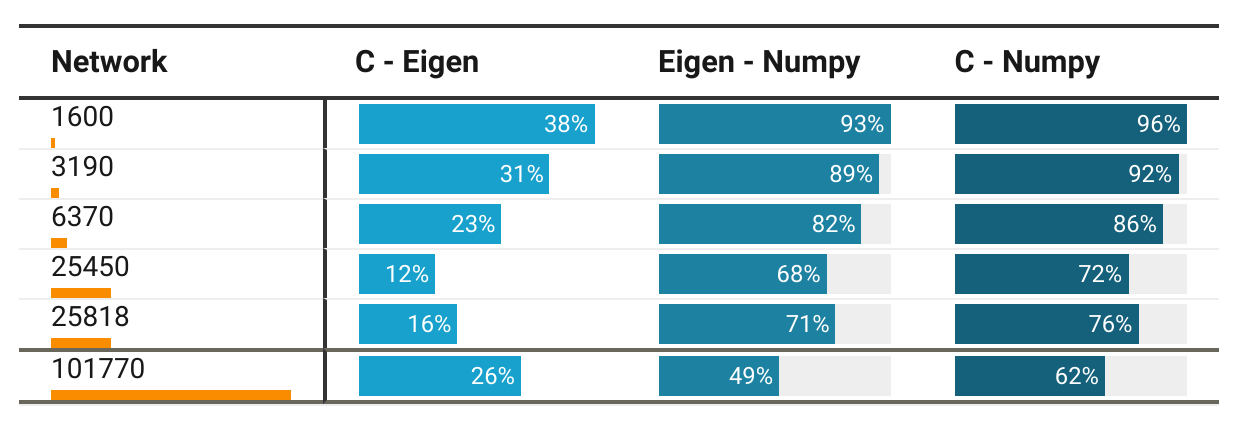
\includegraphics[scale=0.40]{exec_time_comparisons}
	\caption[Execution Time vs Model Parameters]{Percentage difference in accuracies between the implementations.}
	\label{fig:comparison-exec-time}
\end{figure}

\begin{figure}[ht]
	\centering
	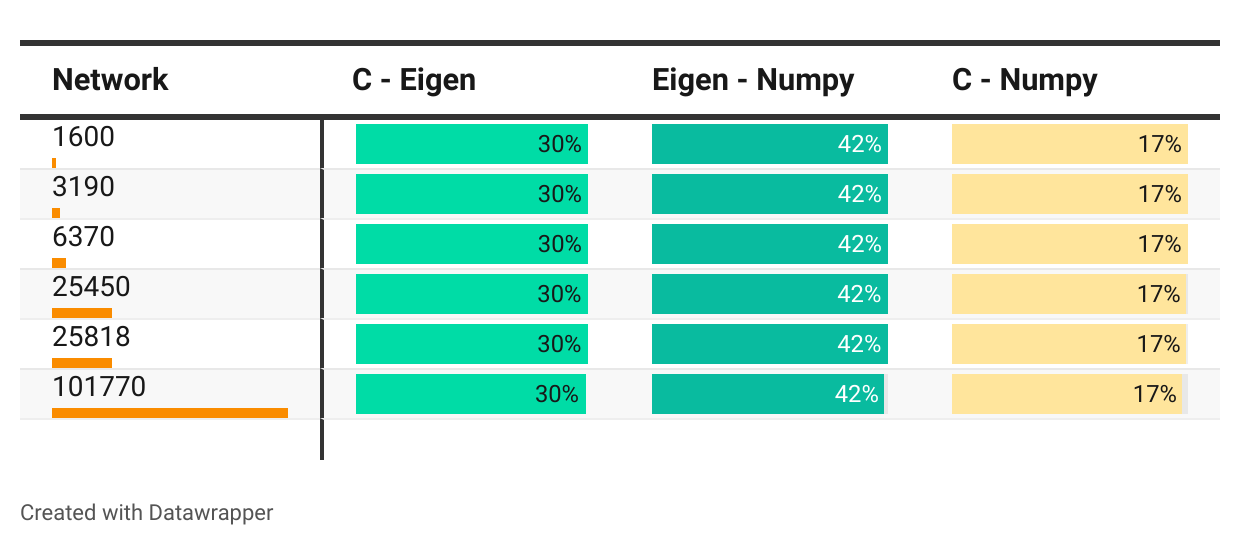
\includegraphics[scale=0.30]{peak_memory_comparisons}
	\caption[Peak Memory Utilisation]{Percentage difference in peak memory utilized between the implementations}
	\label{fig:comparison-peak-memory}
\end{figure}

Figures \ref{fig:comparison-exec-time} and \ref{fig:comparison-peak-memory} show the comparison between \texttt{C}-\texttt{C++} Eigen, \texttt{C++} Eigen-\texttt{Python} Numpy and \texttt{C}-\texttt{Python} Numpy. It is calculated as the percentage of 1 - ($\frac{x}{y}$) where $x$ is performance value of the application which has lower value and $y$ is performance value of the application that has higher number.

\subsection{C vs Eigen}

For smaller models, \texttt{C} exhibits superior speed over Eigen (e.g., 38\% faster for a network size of 1600). As the model complexity grows, \texttt{C++} Eigen's performance surpasses \texttt{C}, with execution time differences less than 15\%. However, there are noticeable differences that emerge at larger network sizes. Both the \texttt{C} and \texttt{C++} Eigen proves 26\% faster than Eigen. Further investigation is needed to pinpoint the source of this anomaly. Eigen excels in memory utilization, outperforming \texttt{C} by 30\%.

\subsection{C vs Numpy}

Notably, \texttt{C} consistently outperforms Numpy. In the case of a network size of 101,770, \texttt{C} exhibits a remarkable 62\% speed advantage. Numpy, however, consumes 17\% more runtime memory compared to \texttt{C}.

\subsection{Eigen vs Numpy}

Similar to the \texttt{C} comparison, Eigen consistently outpaces Numpy across various network sizes, maintaining similar speed differentials. Eigen shines in memory efficiency, surpassing Numpy by 42\%.

\section{Developer Experience}

Embedded environments are greatly varied and working on these platforms are different compared to the more general platforms with comparably reduced support. The greatest challenge in writing the benchmark applications were in sourcing the binaries for the general purpose neural network frameworks. Both Tensorflow and PyTorch do not target the ARMv7 environment that was the primary target for this project. The older community tensorflow binaries that are available for the platform are currently unmaintained, at the time of writing this report. Finally, the PyTorch source code was successfully compiled for our target environment using QEMU user-mode emulation.

The embedded hardware and software ecosystems are greatly varied and fragmented leading to less support from the machine learning software ecosystem. The embedded machine learning communities largely contain sprawling technologies that have several components that have varying degrees of maintenance and create complicated interrelationships over time that are difficult or unwieldy to maintain. This has lead to a lack of good software infrastructure that can support multi-hardware, multi-architecture neural network frameworks.

\subsection{Reverse Engineering Scania ECU}

Scania ECU operating system environment is provided by its system maker without providing access to the Board/SoM fork. The boot sequence divulges minimal information, leading to the difficulties in providing a separate porting of a customized Embedded Linux. The device comes primarily in the form of a custom encased hardware, housing Ethernet over modem and a UART interface. A supplementary hardware circuit schematic document along with certain factory reset scripts adds some information. Regrettably, the information regarding processor specifications, memory unit, bootloader specifics, the boot sequence, and of its peripherals remained elusive.

The absence of development tools on the device itself strips away the convenience of on-device programming. The basic functionality of executing common commands that would yield insights into the system's inner workings has been stymied by intentional disabling of several features on the bootloader and kernel.

Key details such as the processor type, architecture specifications, input/output interfaces on the board, and the essential boot flow process were extracted successfully. Similarly, valuable software information, such as bootloader specifics, the kernel and compiler details, the C library version was also obtained. Information about the memory layout and the device tree configuration however was not obtained.

NXP's Serial Download Mode (SDM) is a specialized mode of operation of the processor on the Scania ECU. SDM allows the processor to be programmed or flashed with new firmware through a serial communication interface, such as UART. Booting the ECU under normal circumstances compared to booting it through SDM revealed unreliable behaviour in the device and several failure modes. The attempts during several iterations rendered the ECU non-operational, a state colloquially referred to as being "bricked". The scarcity of available boards during the project period further made the experimentation process difficult.

The process of flashing within a regular boot sequence was constrained by the absence of development tools. The scope reduced to replacing the bootloader with the MTD partition and with the intention of accessing the bootloader shell. Failures during this phase could be attributed to a plethora of factors: erroneous u-boot images, inconsistencies within the device tree configuration, discrepancies between the versions of the bootloader and kernel, checksum mismatches, or complications arising from oversized files overwriting critical memory regions. The precise cause could not be identified, as there were no logs enabled during the board's booting process.

In the next phase, the ECU was put into SDM. Successful flashing hinged on procuring precise information regarding the memory load addresses and entry points for essential components like the bootloader, kernel and root file system. These crucial details remained elusive, casting a shadow over the feasibility of the flashing process.

Appendix \hyperref[rtc-c300]{I} contains a summary of the efforts involved in reverse engineering the Scania ECU. The project focus shifted to the MCIMX6Q-SDB board after having spent considerable time on the board.

\section{General Distribution of Work}

The reverse engineering efforts were done in unison between the authors by suggesting then attempting different ideas, with Deepak Venkataram working on soldering and other physical manipulations on the Scania ECU. The programming of the benchmark applications was completed by Prasanth Thomas Shaji while the testing of these applications on the MCIMX6Q-SDB were completed by Deepak Venkataram. The primary responsibilities of most activities were divided between the authors however they were performed in concert where possible. The benchmark applications and the report are version controlled in two separate repositories containing commits from both authors and provides the primary accounting of the distribution of work.

\chapter{Conclusion and Future Work}

Developing of neural network implementations for the embedded environment is considerably more challenging than a traditional general purpose personal computer or server computers. The lack of support of on these platforms for the traditional machine learning frameworks stems from the fragmented nature of the embedded ecosystem. There are several challenges in the way for developing a machine learning framework for embedded devices. The current mature frameworks have some means of providing inference passes on embedded platforms however training on-board is still limited to larger platforms.

The development and testing of the benchmark application HDR-NN revealed the difficulties in targetting the \texttt{armv7hl} architecture. The performance of the benchmark applications showed that PyTorch had considerably higher performance than expected for larger shapes than the hand made \texttt{C} implementation. This could however change by working on performance engineering of the \texttt{C} implementations. However, leveraging tool support for performance engineering on these systems are still difficult and requires heavy investment in time.

\section{Future Work}

The initial mandate on the project was to repurpose the Scania ECU to provide a means of targetting the platform reliably. There are yet more technical hurdles to achieving that goal. On-Board Training of neural network models is an active area of reach in TinyML with several efforts in both academia and industry to achieve efficient training algorithms.

\subsection{Porting to Scania ECU}

Repurposing the Scania ECU is a technical challenge that was left incomplete during the project. The experience as detailed in Appendix \hyperref[rtc-c300]{II} and throughout the report. The attempt concluded without having ported the Embedded Linux onto the board. Further information on the device tree layout may be extracted by leveraging the \texttt{/proc/device-tree} Linux interface and a binary disassembly of the bootloader on-board the device could reveal more information about the memory layout. These efforts were dropped in favour of continuing the work on the MCIMX6Q-SDB.

\subsection{On Device Training}

Multi-framework software infrastructure that allows On Device training are being developed by the community in parts such as Modular \cite{mojo}, EdgeImpulse, etc. There are innovative approaches to bring down the memory requirements of deep learning neural network models such as the Tiny Training Engine \cite{lin2022ondevice} and TinyTL \cite{cai2021tinytl} by changing the learning algorithm that will be running on-board.

The fundamental bottleneck of implementing neural network training is the amount of memory required. The memory requirements for training a neural network is larger than for neural network inference due to the requirement for storing intermediate activations of the neural network layers. The backpropagation algorithm requires these intermediate calculations of these values to be present while executing the backward pass. Ideas that work for implementing efficient neural network inference on embedded hardware, such as improving parameter efficiency by reducing the number of parameters in the neural network model, do not work to bring down on the total number of activations values required to be stored during the training process.
